\section{\MakeUppercase{Результати бібліометричного аналізу}}
\label{sec:chapter2}

\subsection{Описова статистика вибірки}
\label{sec:descriptive_stats}

Вибірка з 1998 публікацій бази Web of Science Core Collection охоплює період з 1997 по 2025 рік. Аналіз динаміки публікацій (рис.~\ref{fig:pub_years}) показує стале зростання кількості досліджень із моніторингу ПТО, з найвищою активністю у 2019--2023 роках. Це відображає зростаючий інтерес наукової спільноти до проблем якості та моніторингу професійної освіти, зафіксований у звітах міжнародних організацій~\cite{OECD2010, CedefopReport2017, Cedefop2020, UNEScounevoc2013}.

\begin{figure}[htbp]
    \centering
    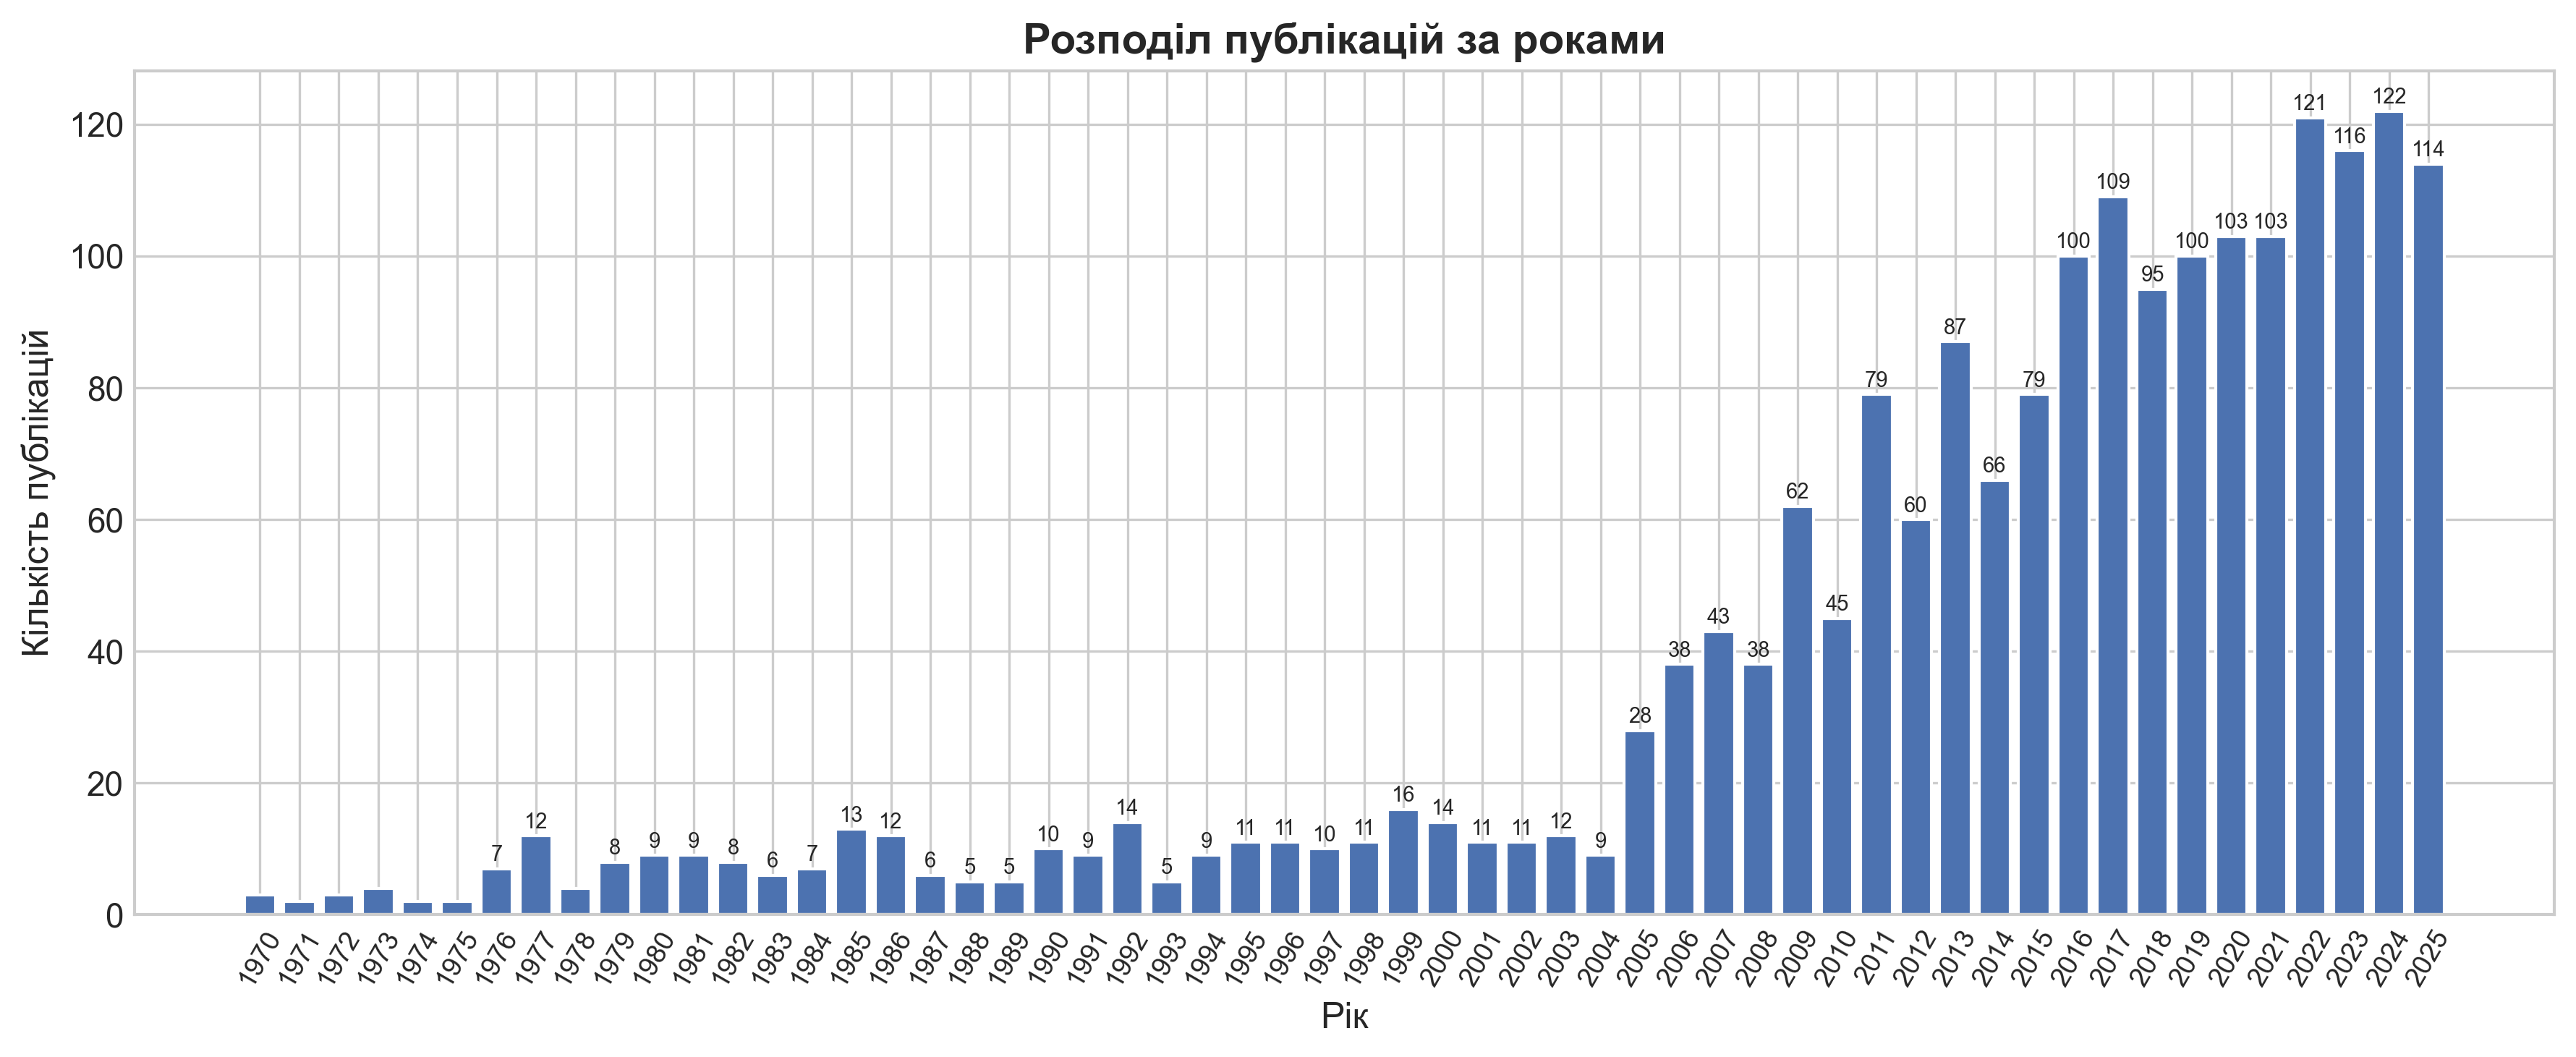
\includegraphics[width=\linewidth]{media/fig_pub_years.png}
    \caption{Розподіл публікацій за роками (1997--2025).}
    \label{fig:pub_years}
\end{figure}

За типами документів (рис.~\ref{fig:doc_types}) переважають наукові статті (articles), що свідчить про зрілість дослідницького поля. Значну частку також складають матеріали конференцій (proceedings papers), що вказує на активний обмін результатами на міжнародних форумах.

\begin{figure}[htbp]
    \centering
    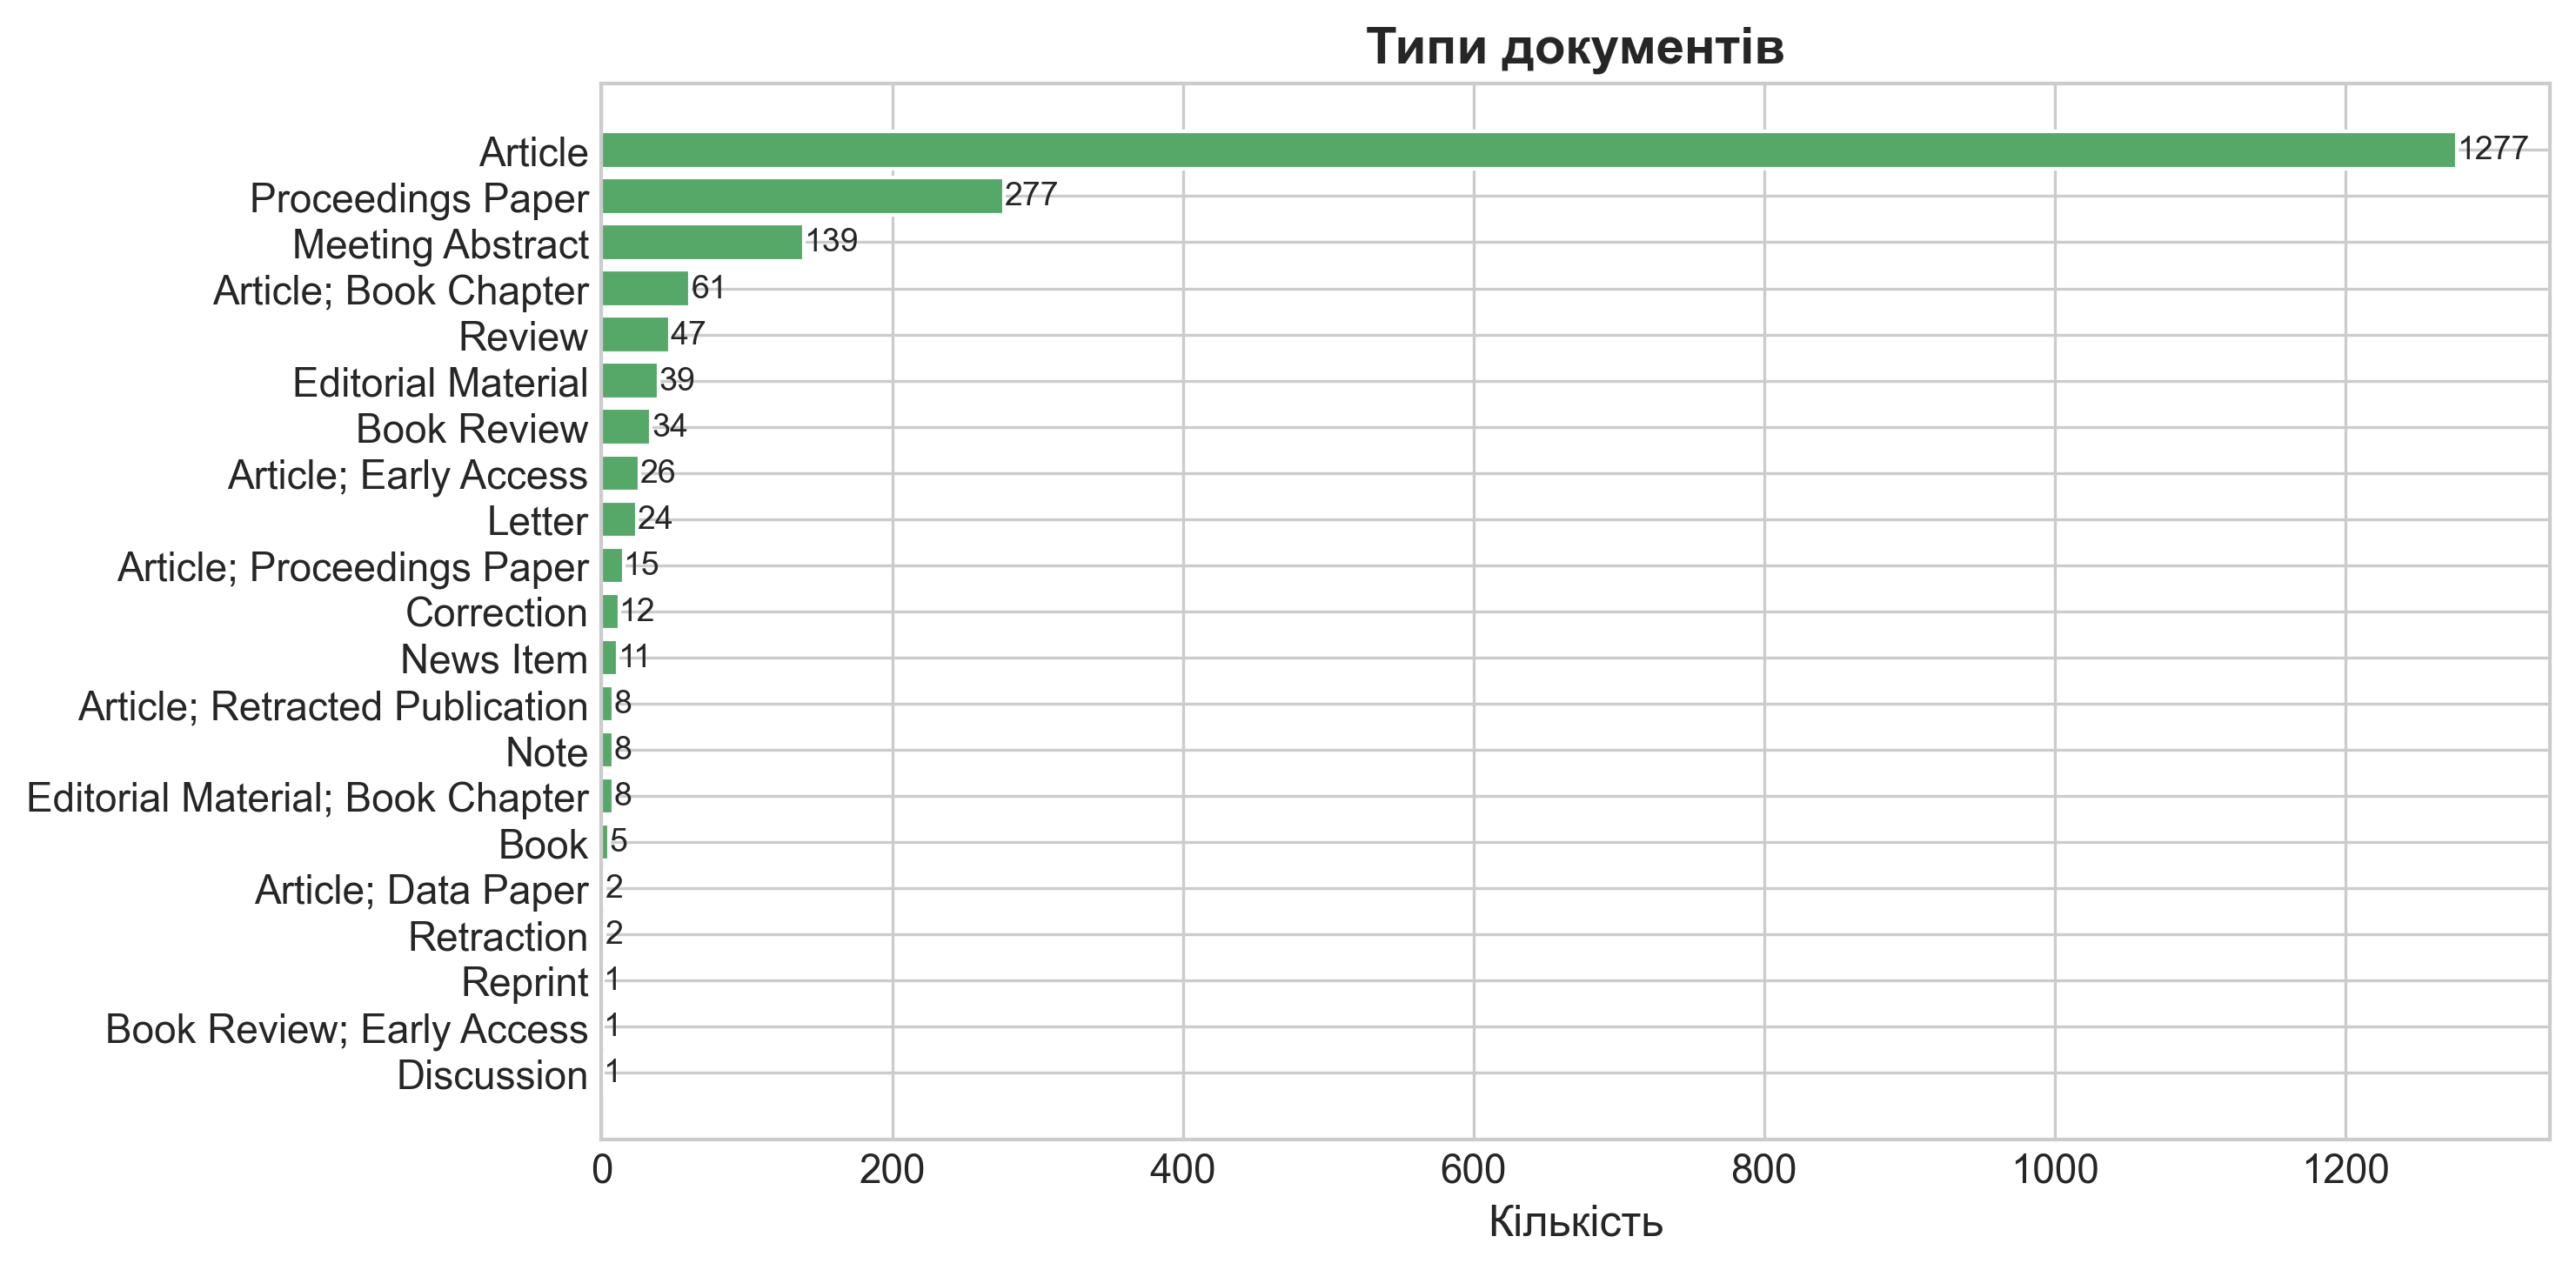
\includegraphics[width=\linewidth]{media/fig_doc_types.png}
    \caption{Розподіл публікацій за типами документів.}
    \label{fig:doc_types}
\end{figure}

Аналіз найбільш продуктивних джерел (рис.~\ref{fig:top_sources}) виявив провідну роль спеціалізованих журналів з професійної освіти, таких як Journal of Vocational Education and Training, Empirical Research in Vocational Education and Training, та International Journal for Research in Vocational Education and Training. Присутність журналів з ширшим охопленням (Education and Training, European Journal of Training and Development) свідчить про міждисциплінарний характер досліджень моніторингу ПТО.

\begin{figure}[htbp]
    \centering
    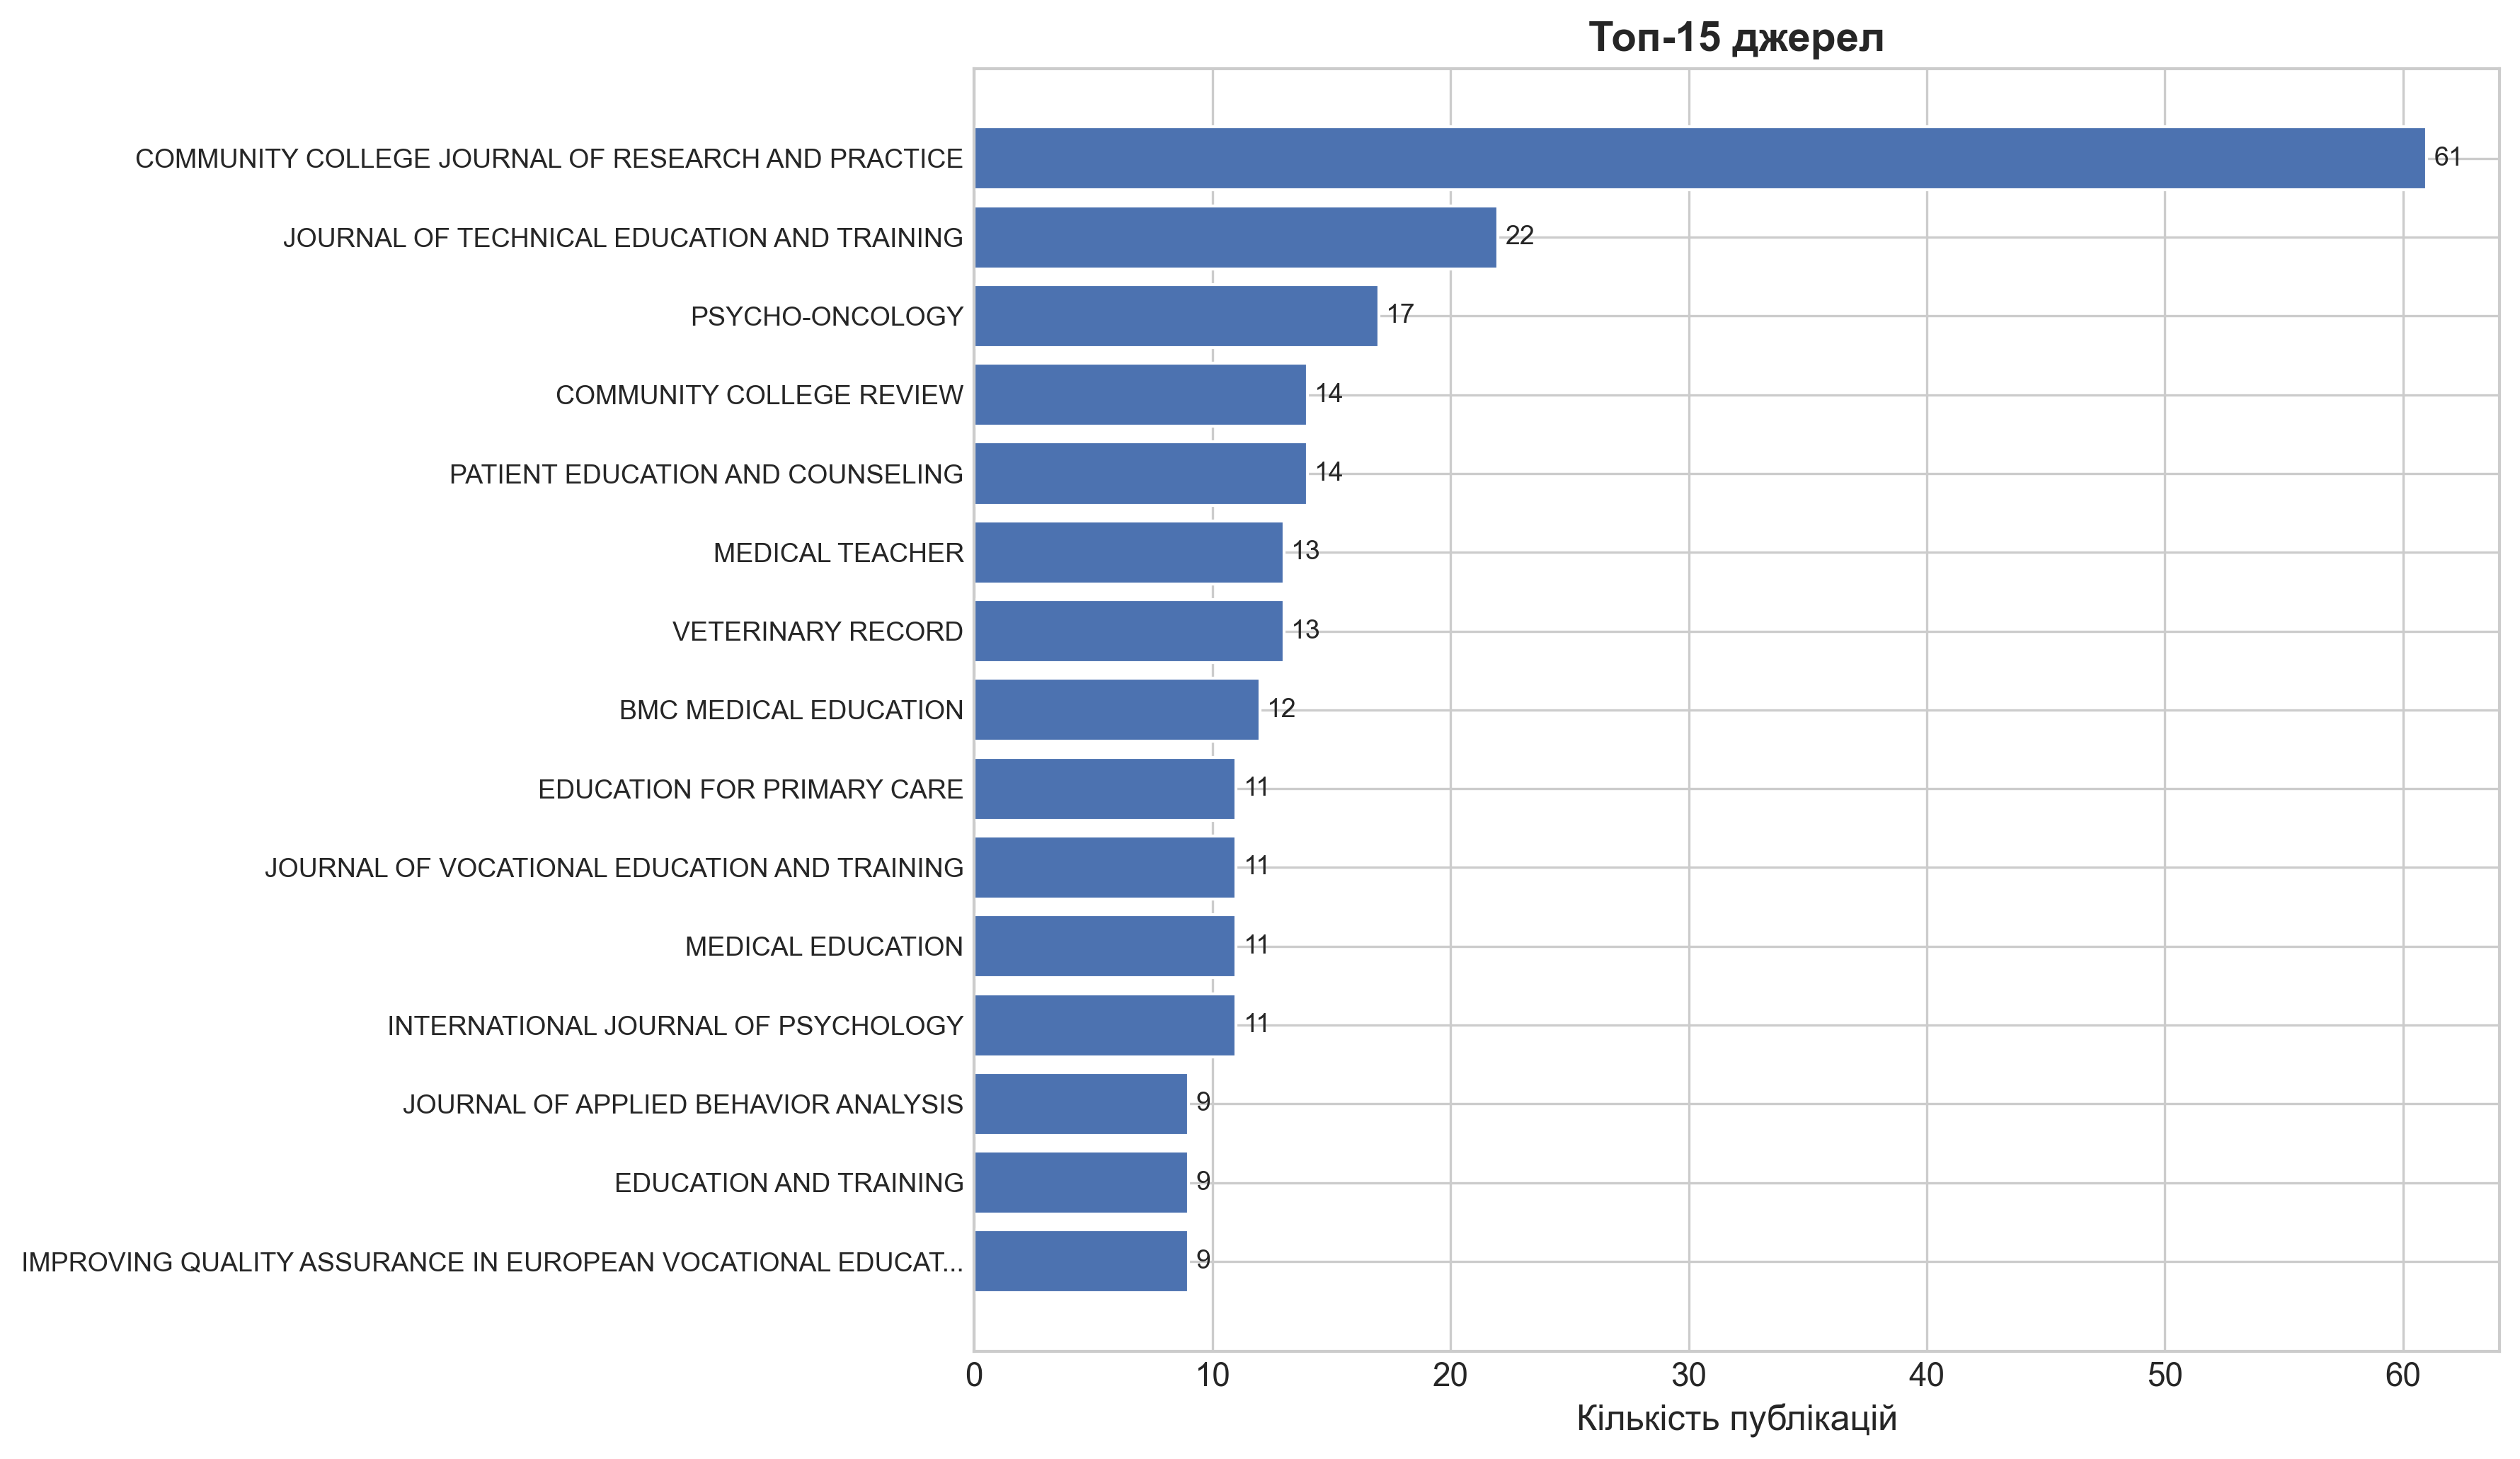
\includegraphics[width=\linewidth]{media/fig_top_sources.png}
    \caption{Топ-15 наукових джерел за кількістю публікацій.}
    \label{fig:top_sources}
\end{figure}

Географічний розподіл авторів (рис.~\ref{fig:top_countries}) демонструє домінування європейських країн, зокрема Німеччини, Нідерландів та Великої Британії, що узгоджується з розвиненою системою дуальної професійної освіти в цих країнах. Присутність Австралії, США та Китаю вказує на глобальний характер досліджень.

\begin{figure}[htbp]
    \centering
    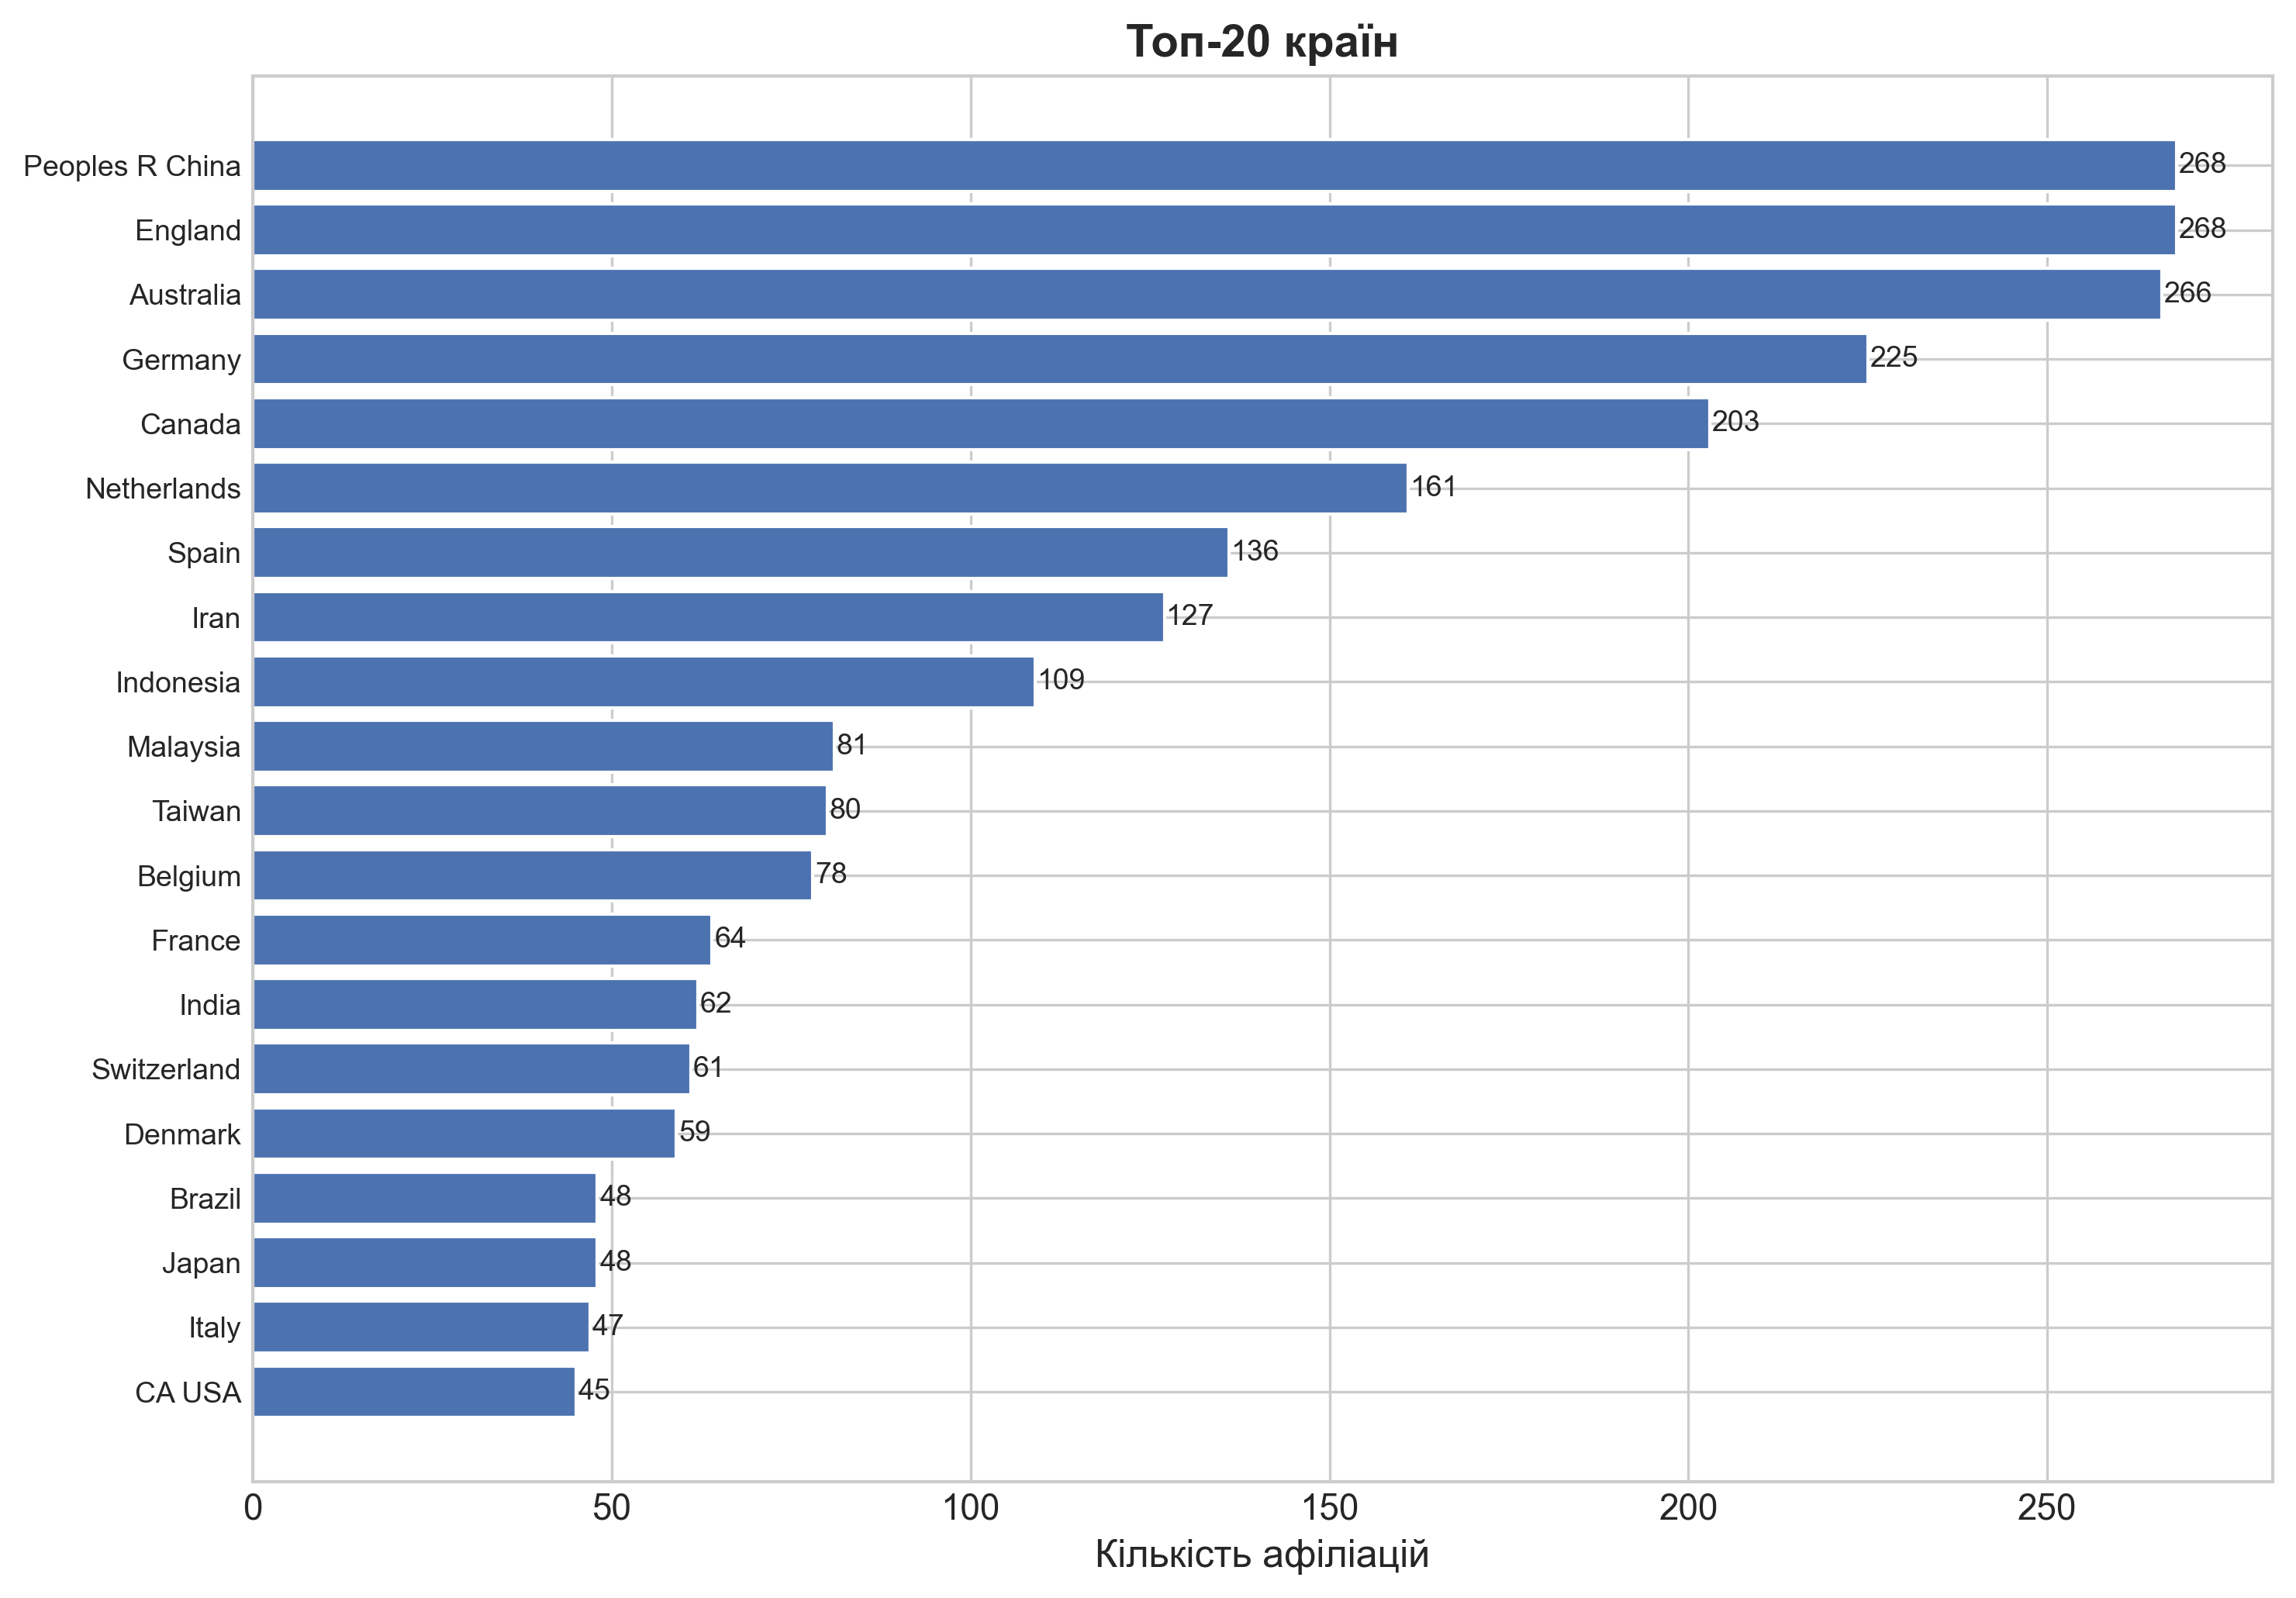
\includegraphics[width=\linewidth]{media/fig_top_countries.png}
    \caption{Топ-20 країн за кількістю публікацій.}
    \label{fig:top_countries}
\end{figure}

Розподіл за авторами (рис.~\ref{fig:top_authors}) дозволяє ідентифікувати найбільш продуктивних дослідників у галузі моніторингу ПТО.

\begin{figure}[htbp]
    \centering
    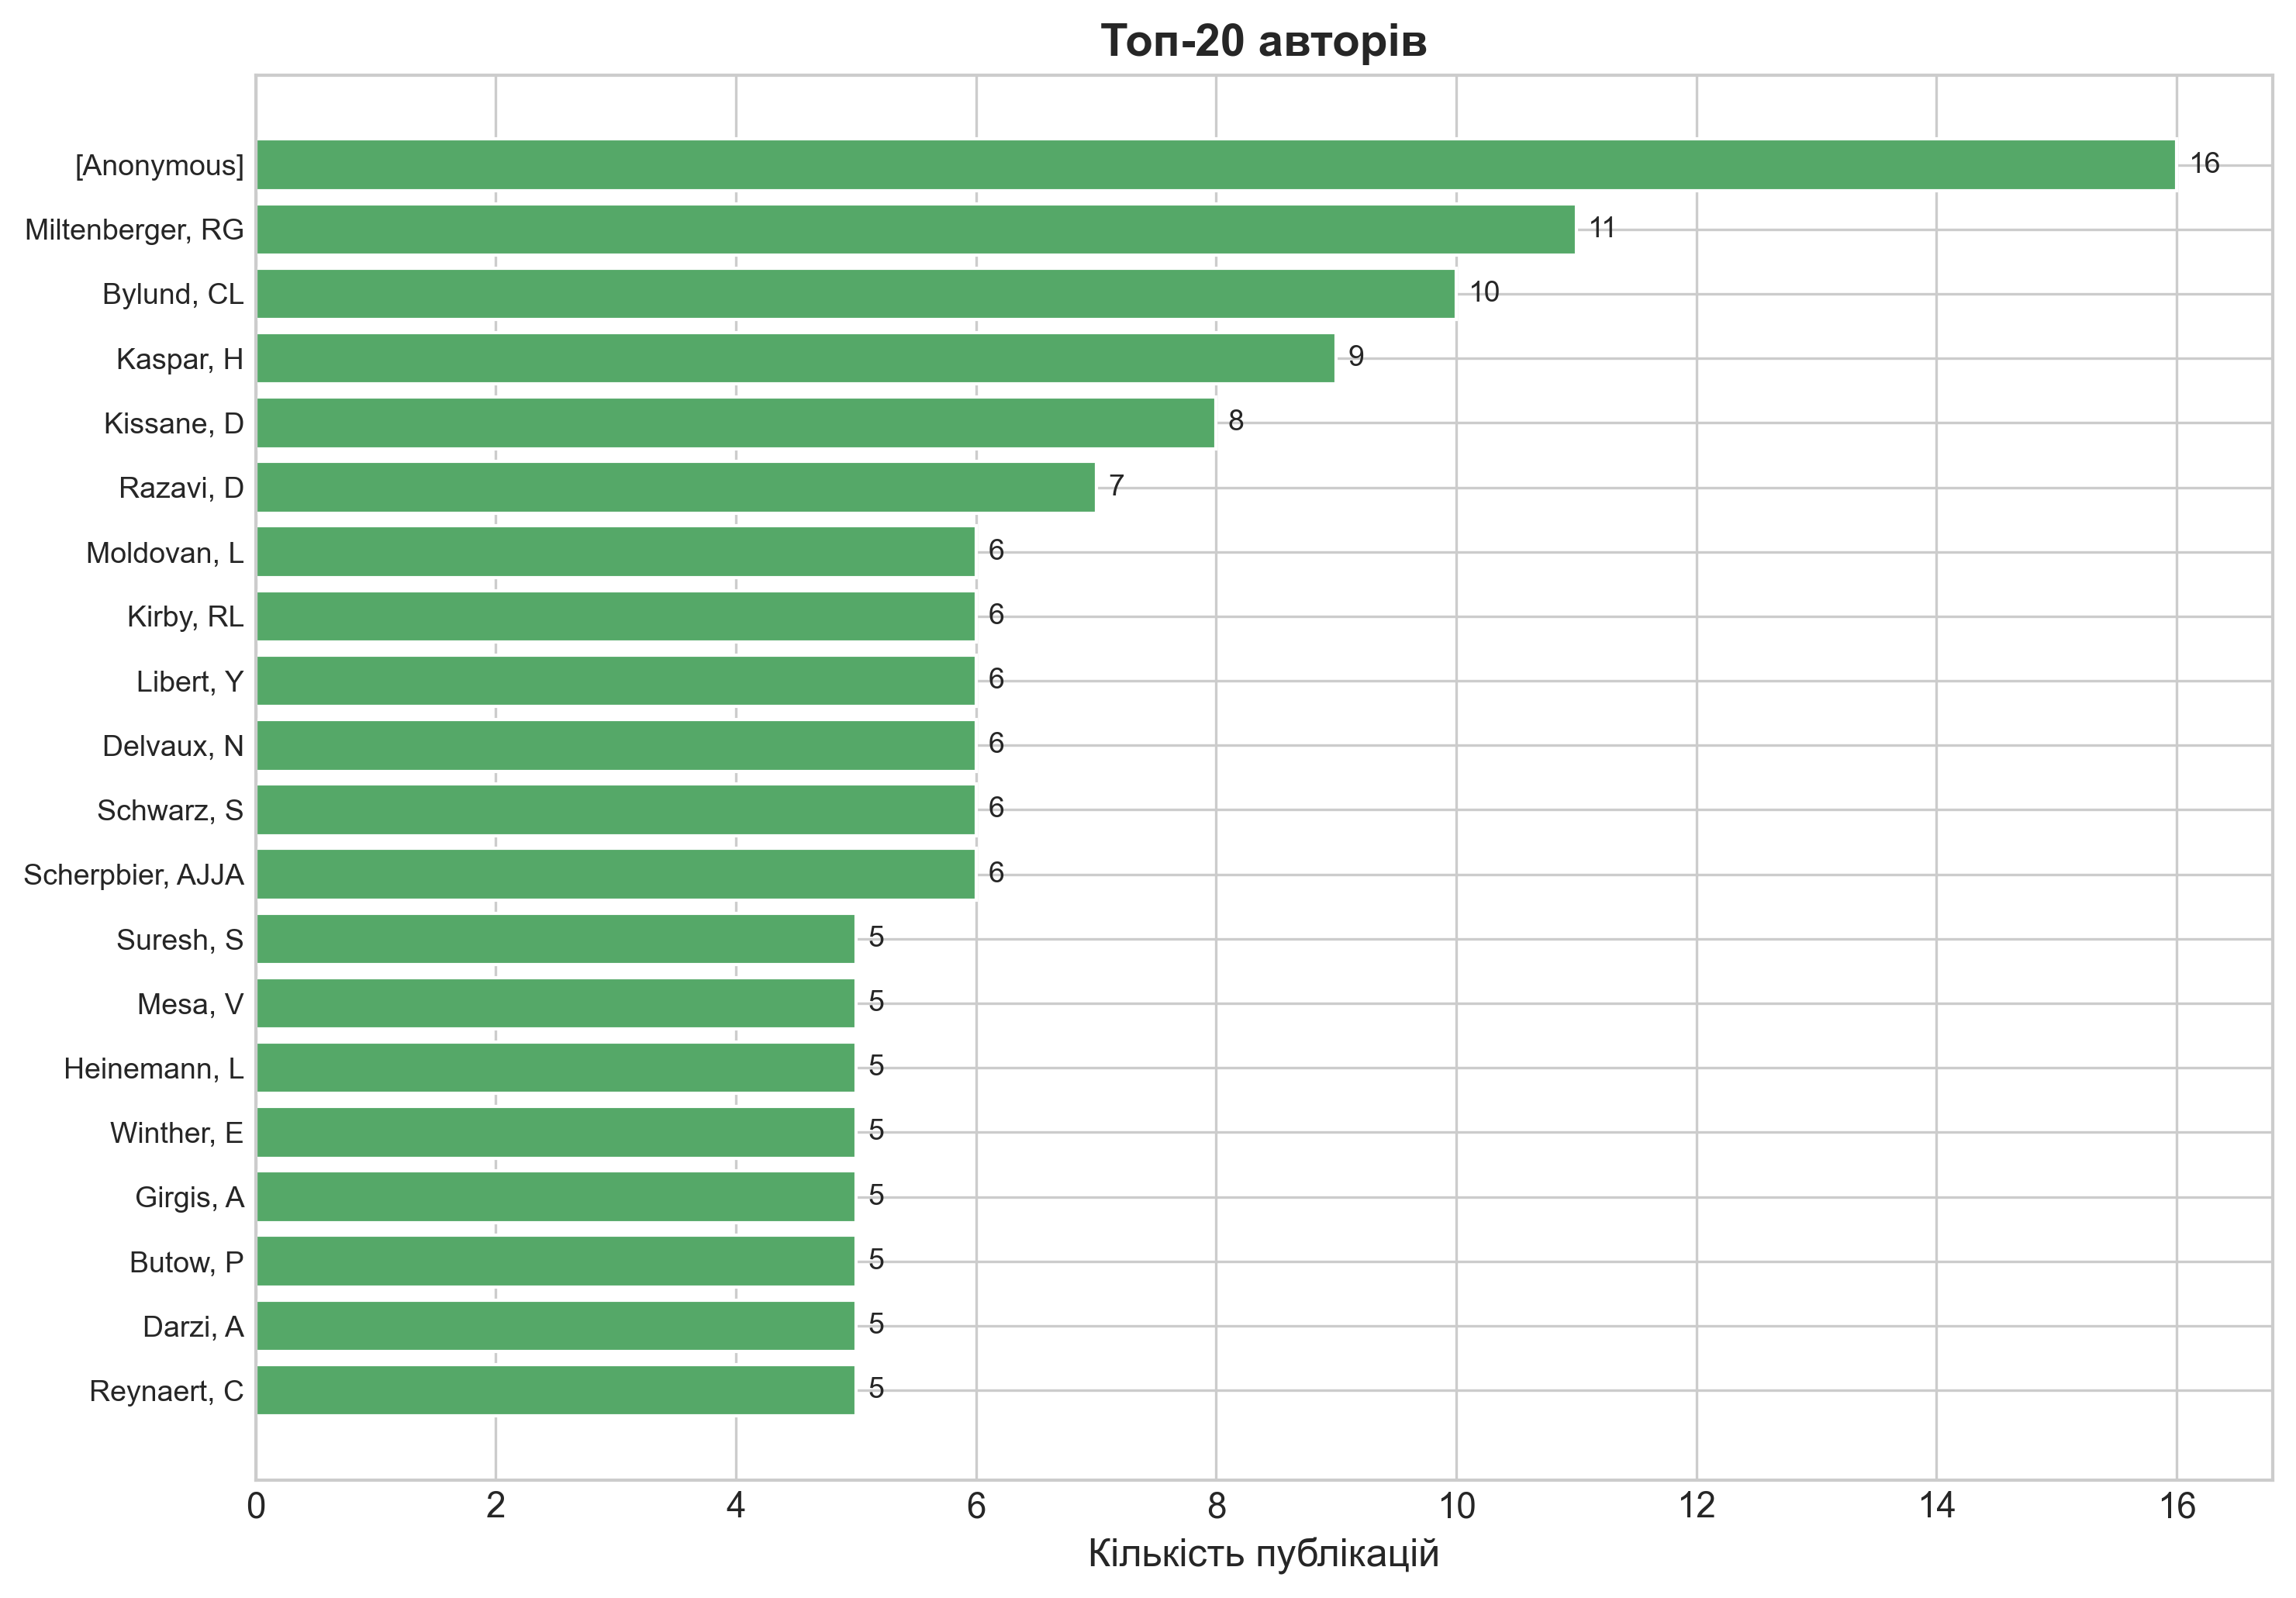
\includegraphics[width=\linewidth]{media/fig_top_authors.png}
    \caption{Топ-20 авторів за кількістю публікацій.}
    \label{fig:top_authors}
\end{figure}

Аналіз авторських ключових слів (рис.~\ref{fig:keywords_de}) показує, що найбільш уживаними є терміни <<vocational education and training>>, <<assessment>>, <<competence>>, <<apprenticeship>>, що відображають ключові теми дослідницького поля. Аналогічний аналіз Keywords Plus (рис.~\ref{fig:keywords_id}), які автоматично присвоюються WoS на основі цитованих посилань, виявляє ширшу тематичну картину з акцентом на <<education>>, <<performance>>, <<quality>> та <<skills>>.

\begin{figure}[htbp]
    \centering
    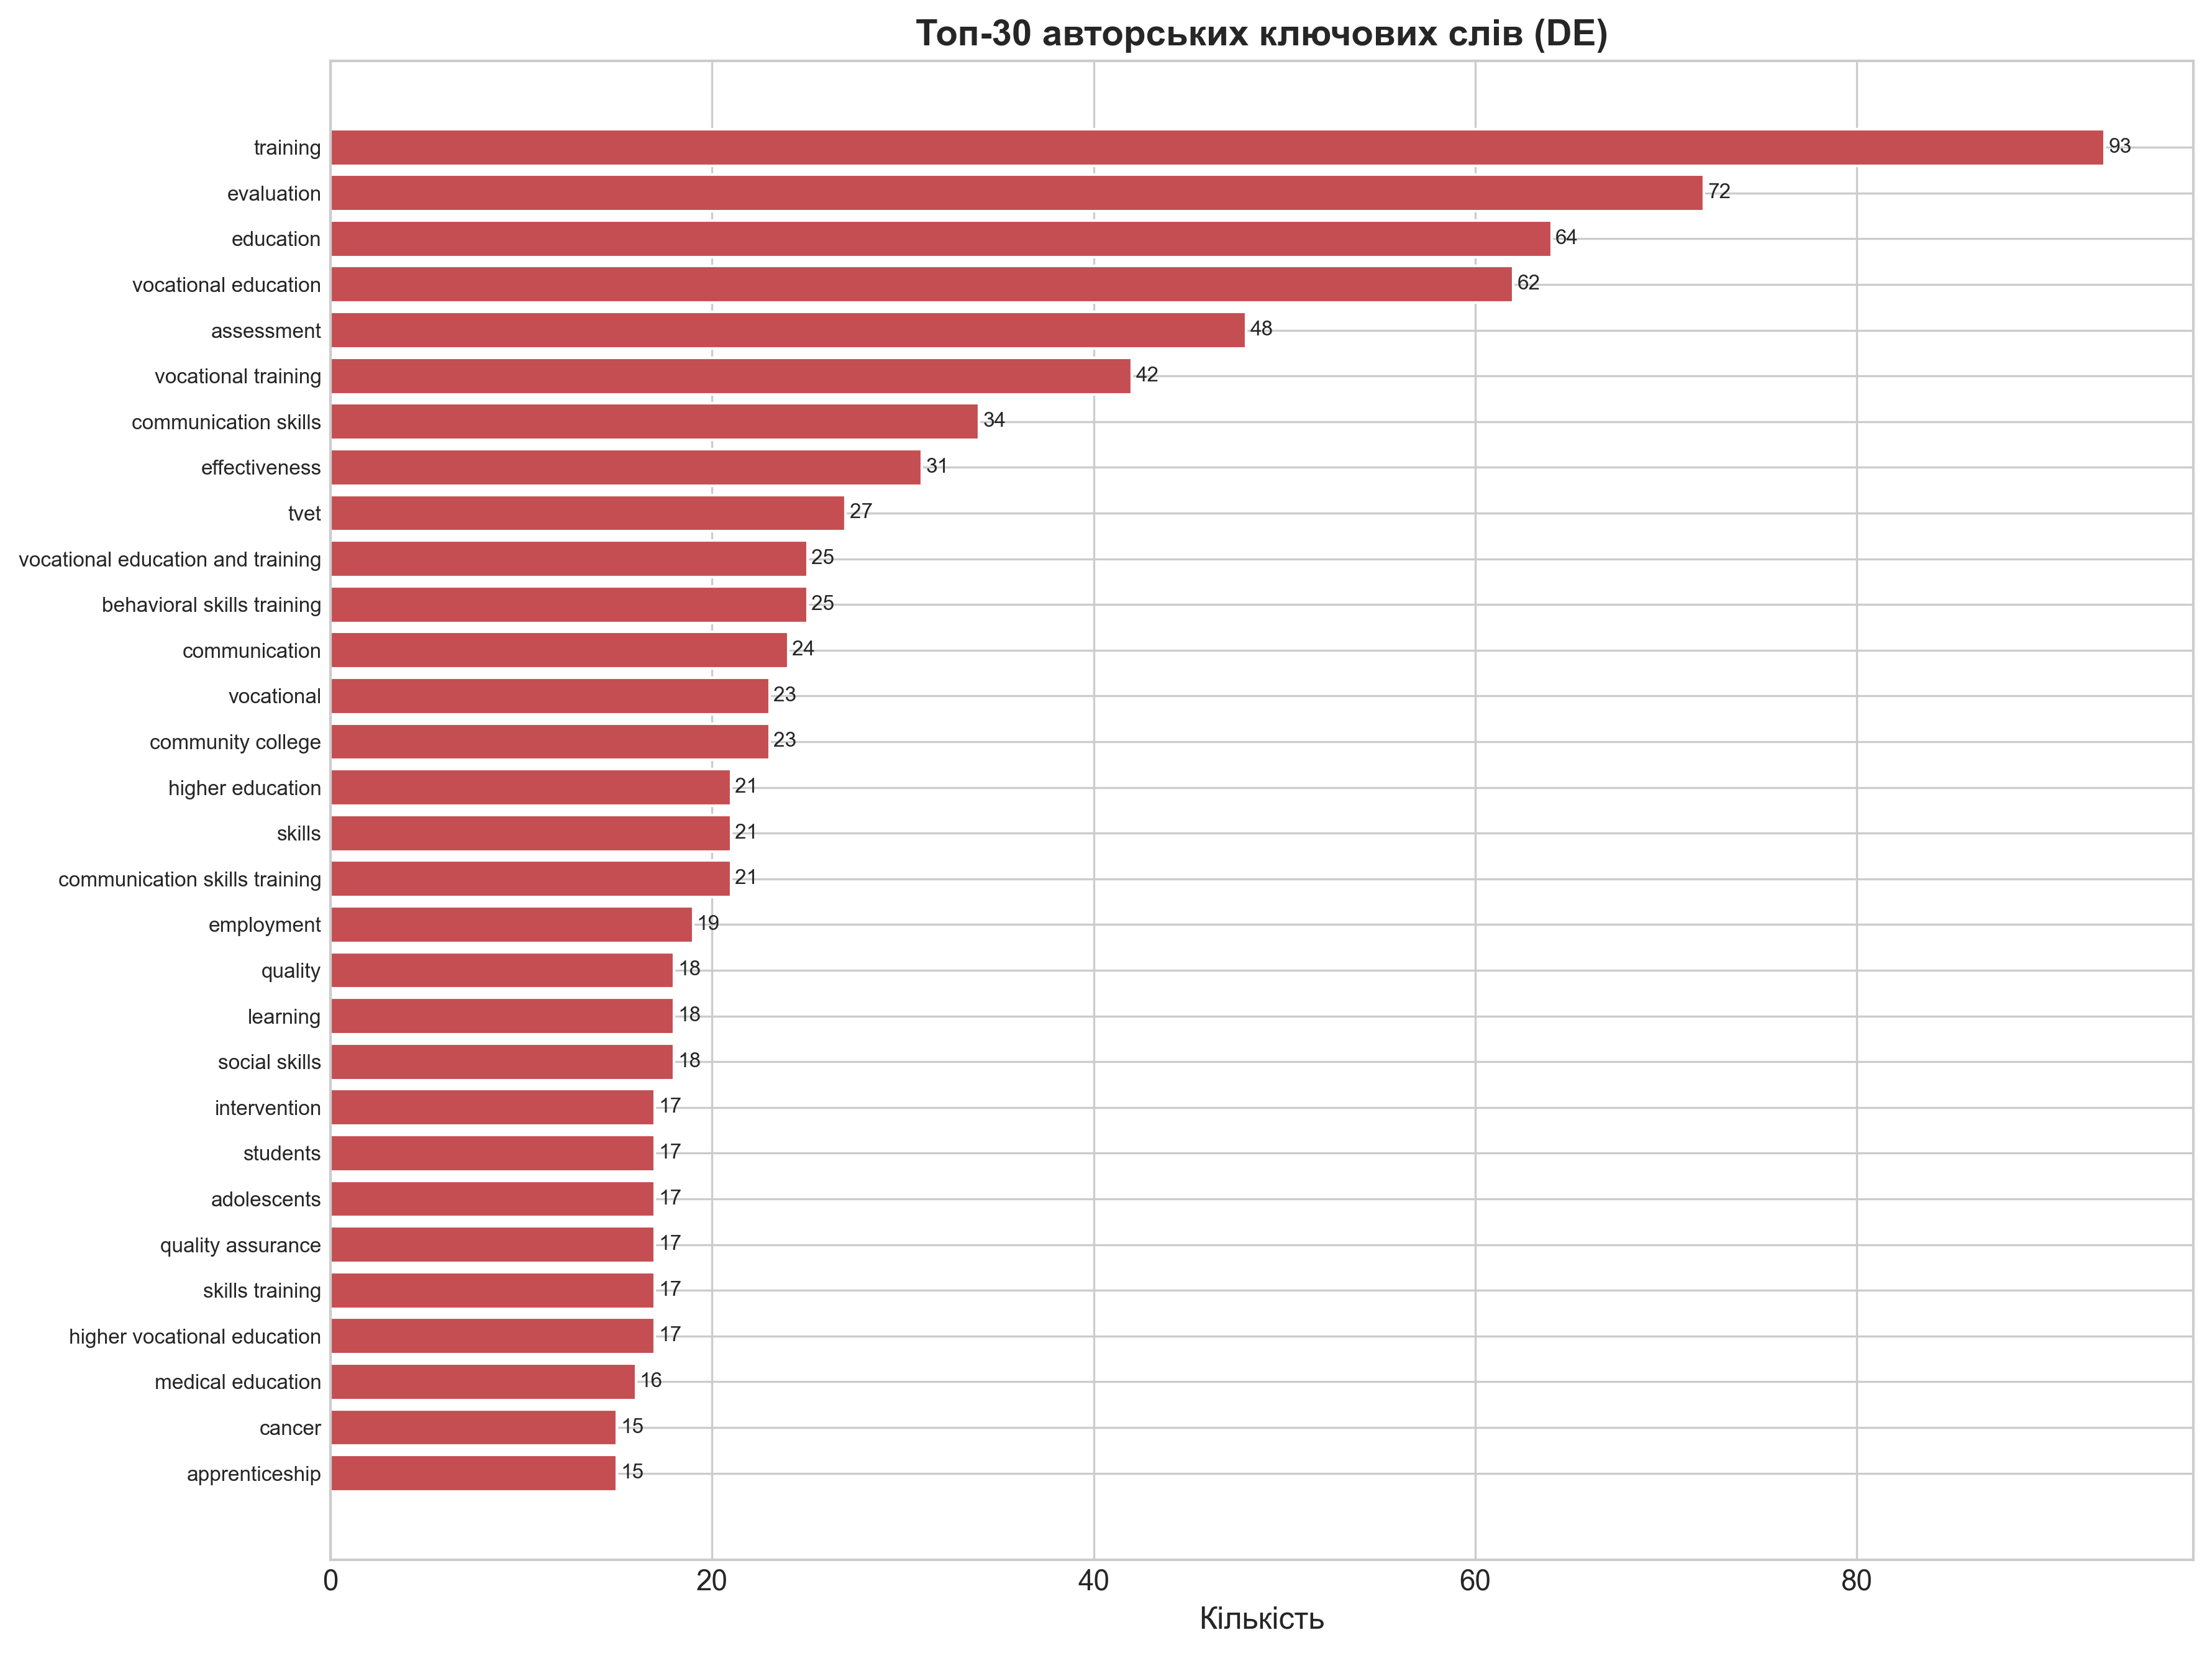
\includegraphics[width=\linewidth]{media/fig_keywords_de.png}
    \caption{Топ-30 авторських ключових слів (DE).}
    \label{fig:keywords_de}
\end{figure}

\begin{figure}[htbp]
    \centering
    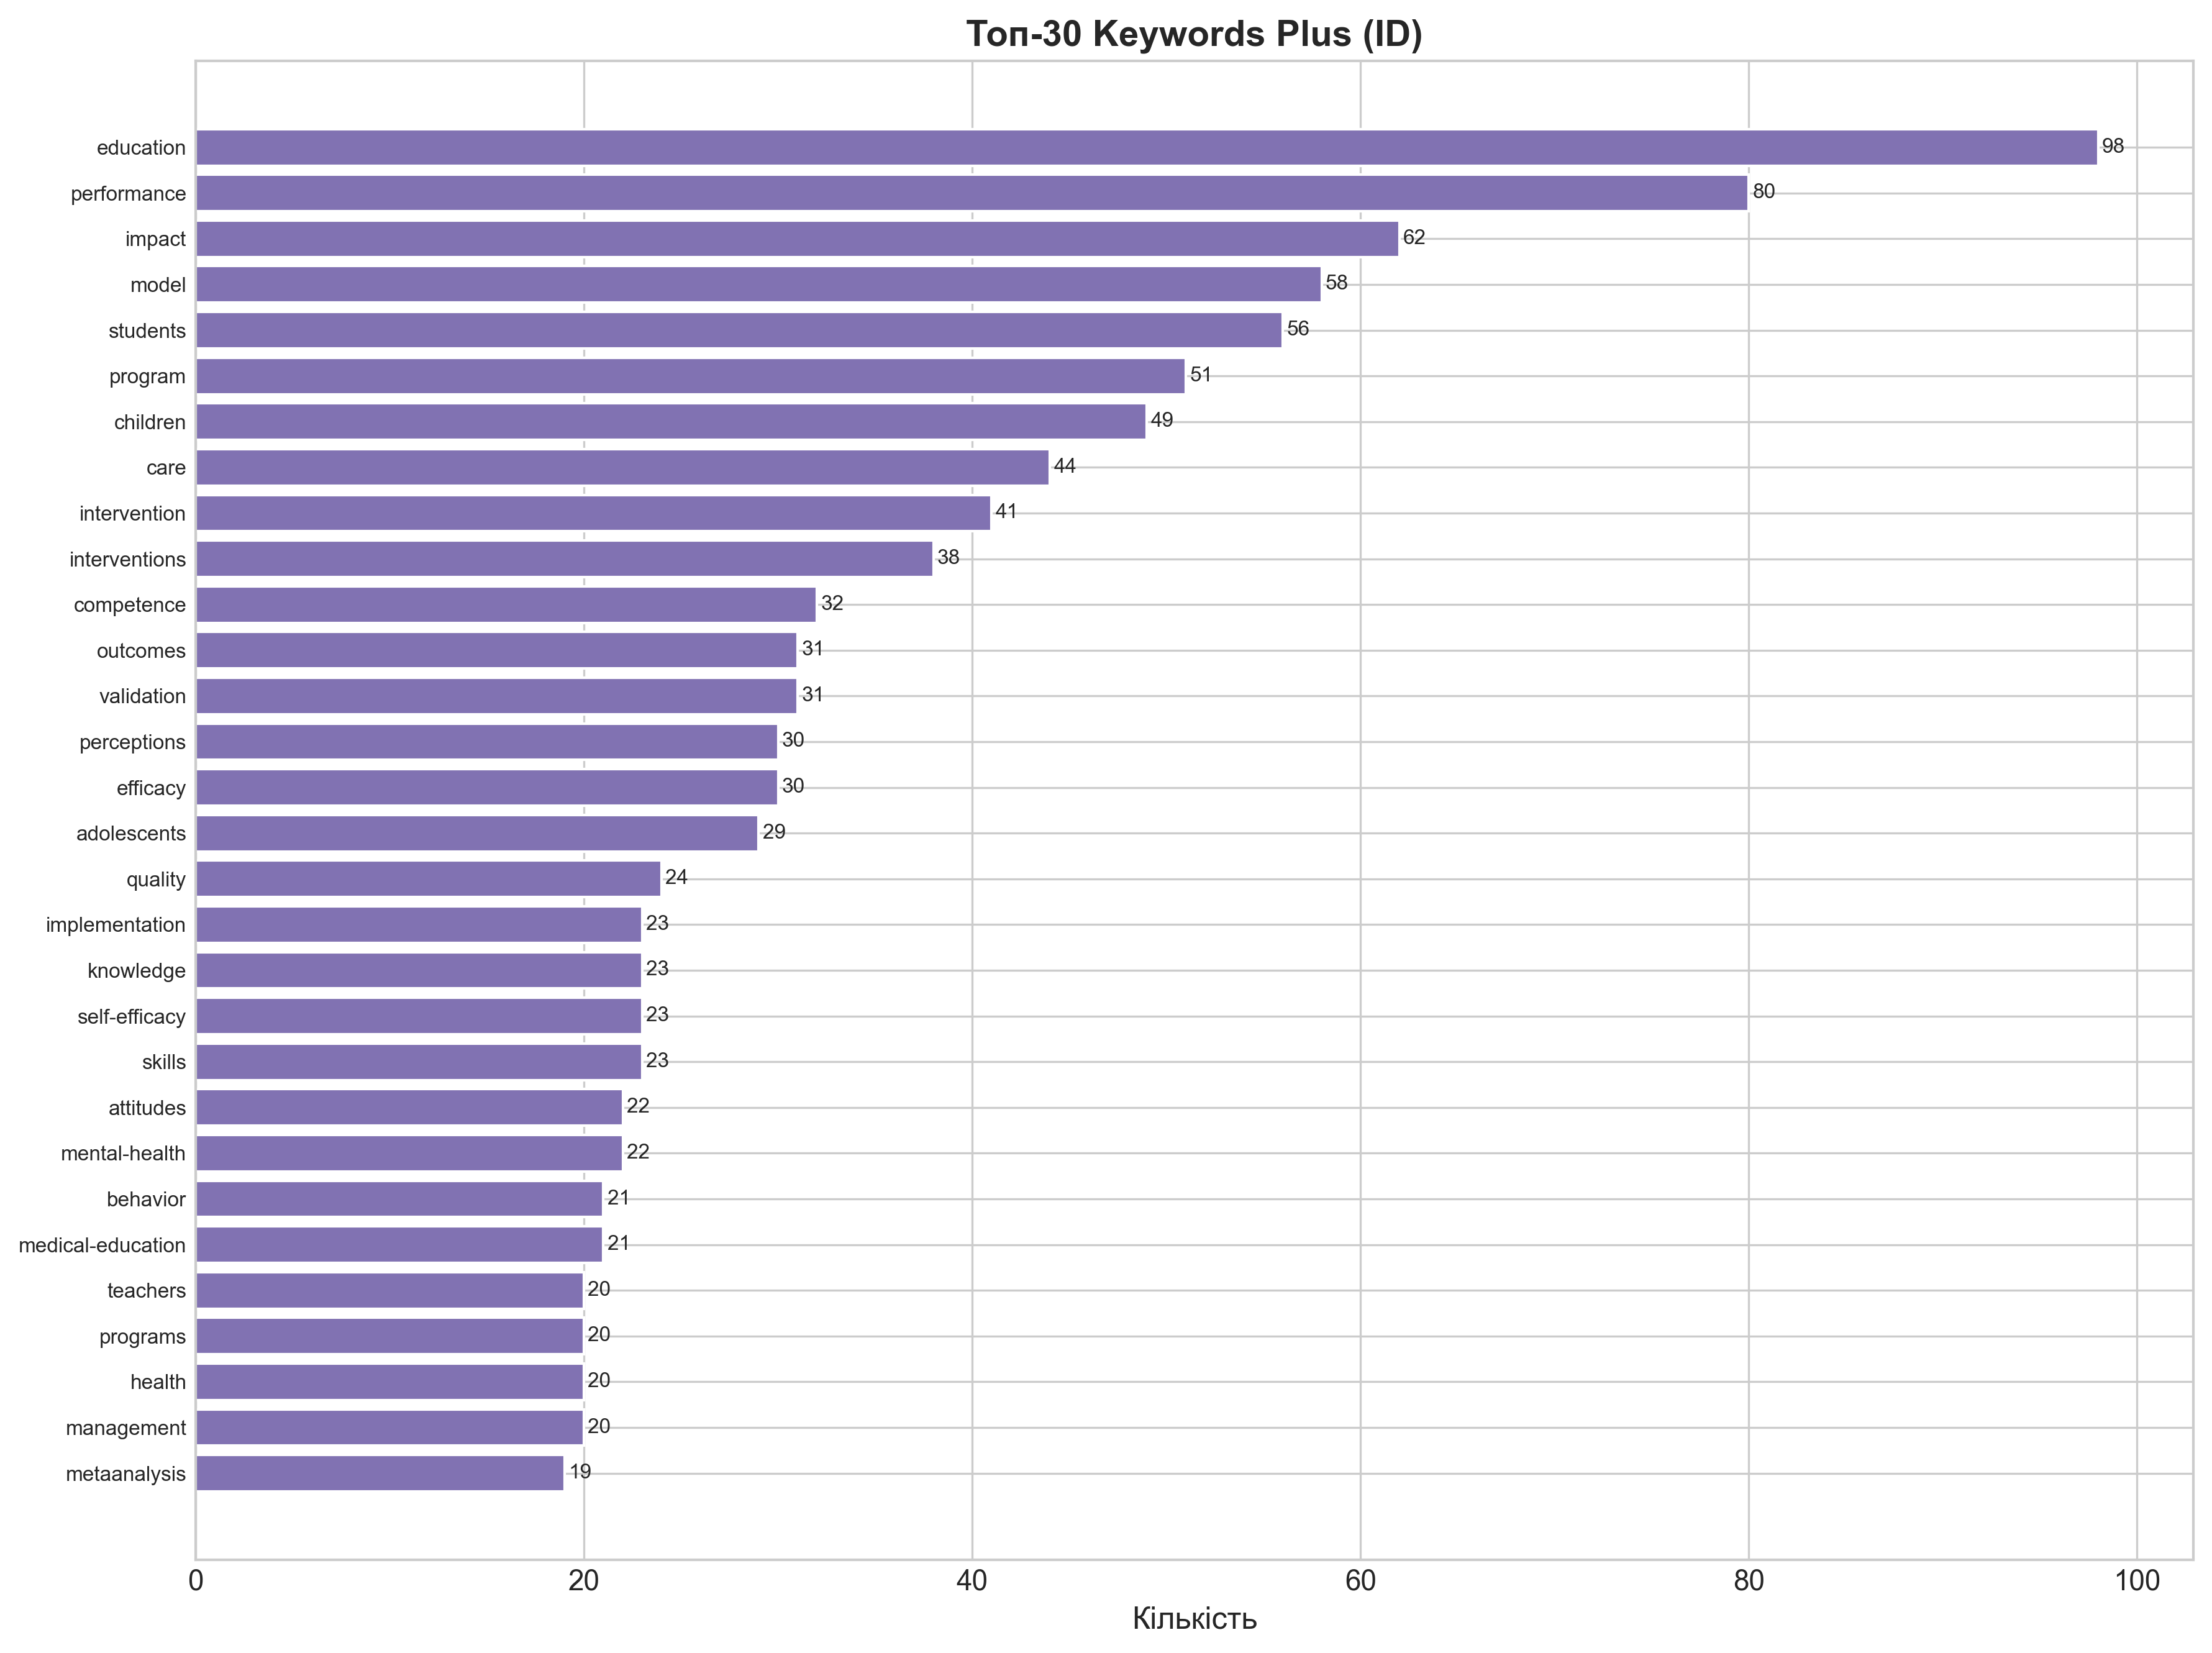
\includegraphics[width=\linewidth]{media/fig_keywords_id.png}
    \caption{Топ-30 Keywords Plus (ID).}
    \label{fig:keywords_id}
\end{figure}

\subsection{Аналіз мережі ключових слів VOSViewer}
\label{sec:vos_network}

На основі текстового аналізу 1000 записів у VOSViewer отримано мережу з 28 ключових слів, розподілених на 4 кластери (табл.~\ref{tab:clusters}).

\begin{table}[htbp]
\centering
\caption{Кластери ключових слів VOSViewer.}
\label{tab:clusters}
\setlength\tabcolsep{3pt}
\begin{tabular}{|c|p{3.5cm}|c|p{8cm}|}
\hline
\textbf{№} & \textbf{Назва кластера} & \textbf{Кількість} & \textbf{Ключові слова} \\
\hline
1 & Системи та політика ПТО & 11 & vet, training, development, model, paper, country, company, field, order, germany, higher education \\
\hline
2 & Результати навчання & 8 & student, study, school, assessment, performance, effect, group, difference \\
\hline
3 & Педагогічна практика & 6 & teacher, competence, practice, learning, work, context \\
\hline
4 & Когнітивні результати & 3 & skill, knowledge, problem \\
\hline
\end{tabular}
\end{table}

\textbf{Кластер~1 <<Системи та політика ПТО>>} є найбільшим і об'єднує 11 термінів. Центральний термін \textit{vet} має найвищу силу зв'язків у всій мережі (TLS\,=\,17\,857). Цей кластер описує інституційний та системний вимір ПТО на макрорівні: порівняльні дослідження національних систем (\textit{country}, \textit{germany})~\cite{Pilz2017, Euler2013}, моделі підготовки кадрів (\textit{training}, \textit{model})~\cite{Busemeyer2012, Bosch2008}, роль роботодавців (\textit{company}), зв'язок із вищою освітою (\textit{higher education})~\cite{Gonon2014}. Термін \textit{company} має найновіший середній рік публікації (2019,85), що свідчить про зростаючу увагу до ролі бізнесу в системі ПТО.

\textbf{Кластер~2 <<Емпіричні дослідження результатів навчання>>} містить 8 термінів, серед яких \textit{student} (TLS\,=\,14\,844) та \textit{study} (TLS\,=\,14\,924) --- два найцентральніші терміни кластера. Кластер відображає емпіричну дослідницьку парадигму: \textit{assessment}, \textit{performance}, \textit{effect} --- класична тріада вимірювання результатів навчання~\cite{Hanushek2017}; \textit{group} та \textit{difference} --- ознаки порівняльного дизайну досліджень~\cite{Eichhorst2015}; \textit{school} --- контекст навчання, включаючи перехід від школи до роботи~\cite{Ryan2001, Aarkrog2005}.

\textbf{Кластер~3 <<Педагогічна практика та компетентнісний підхід>>} об'єднує 6 термінів, зосереджених на процесі навчання та ролі викладача. \textit{Teacher} (TLS\,=\,8\,600) --- центральний актор. \textit{Competence} (TLS\,=\,6\,352) --- ключова концепція сучасної освіти~\cite{Mulder2014}. \textit{Practice}, \textit{learning}, \textit{work}, \textit{context} --- описують зв'язок навчання з реальним професійним середовищем (workplace learning)~\cite{Tynjala2008, Billett2011}. Термін \textit{context} має один із найновіших середніх років (2019,09), що свідчить про зростання уваги до контекстуалізованого навчання.

\textbf{Кластер~4 <<Когнітивні результати та навички>>} --- найменший, але семантично щільний кластер із 3 термінів. \textit{Skill} (TLS\,=\,5\,910) --- центральний результат ПТО~\cite{Rauner2008}. \textit{Knowledge} (TLS\,=\,4\,652) --- когнітивна основа компетентностей~\cite{Winch2010, Wheelahan2010}. \textit{Problem} (TLS\,=\,3\,324) --- вказує на проблемно-орієнтований підхід у навчанні.

Просторове розташування кластерів відображає семантичну структуру дослідницького поля. Горизонтальна вісь X інтерпретується як <<Система~$\leftrightarrow$~Особистість>>: ліворуч розташовані терміни інституційного рівня (\textit{vet}, \textit{training}, \textit{country}, \textit{germany}), праворуч~-- індивідуального рівня (\textit{student}, \textit{teacher}, \textit{skill}, \textit{performance}). Вертикальна вісь Y інтерпретується як <<Результати~$\leftrightarrow$~Процес>>: внизу~-- терміни вимірювання (\textit{effect}, \textit{group}, \textit{difference}), вгорі~-- терміни процесу навчання (\textit{context}, \textit{teacher}, \textit{learning}, \textit{work}).

Найцентральніші терміни всієї мережі~-- \textit{vet}, \textit{study}, \textit{student}, \textit{training}~-- утворюють <<золотий чотирикутник>> досліджень ПТО, що пов'язує системний рівень (vet, training) з рівнем учасників та дослідників (student, study).

\subsection{Мережеві візуалізації}
\label{sec:visualizations}

На рис.~\ref{fig:network_vosviewer} представлено мережу ключових слів, побудовану за координатами VOSViewer, де розмір вузла пропорційний кількості входжень терміна, а колір відповідає кластерній належності. Товщина зв'язків відображає силу ко-входжень між термінами.

\begin{figure}[htbp]
    \centering
    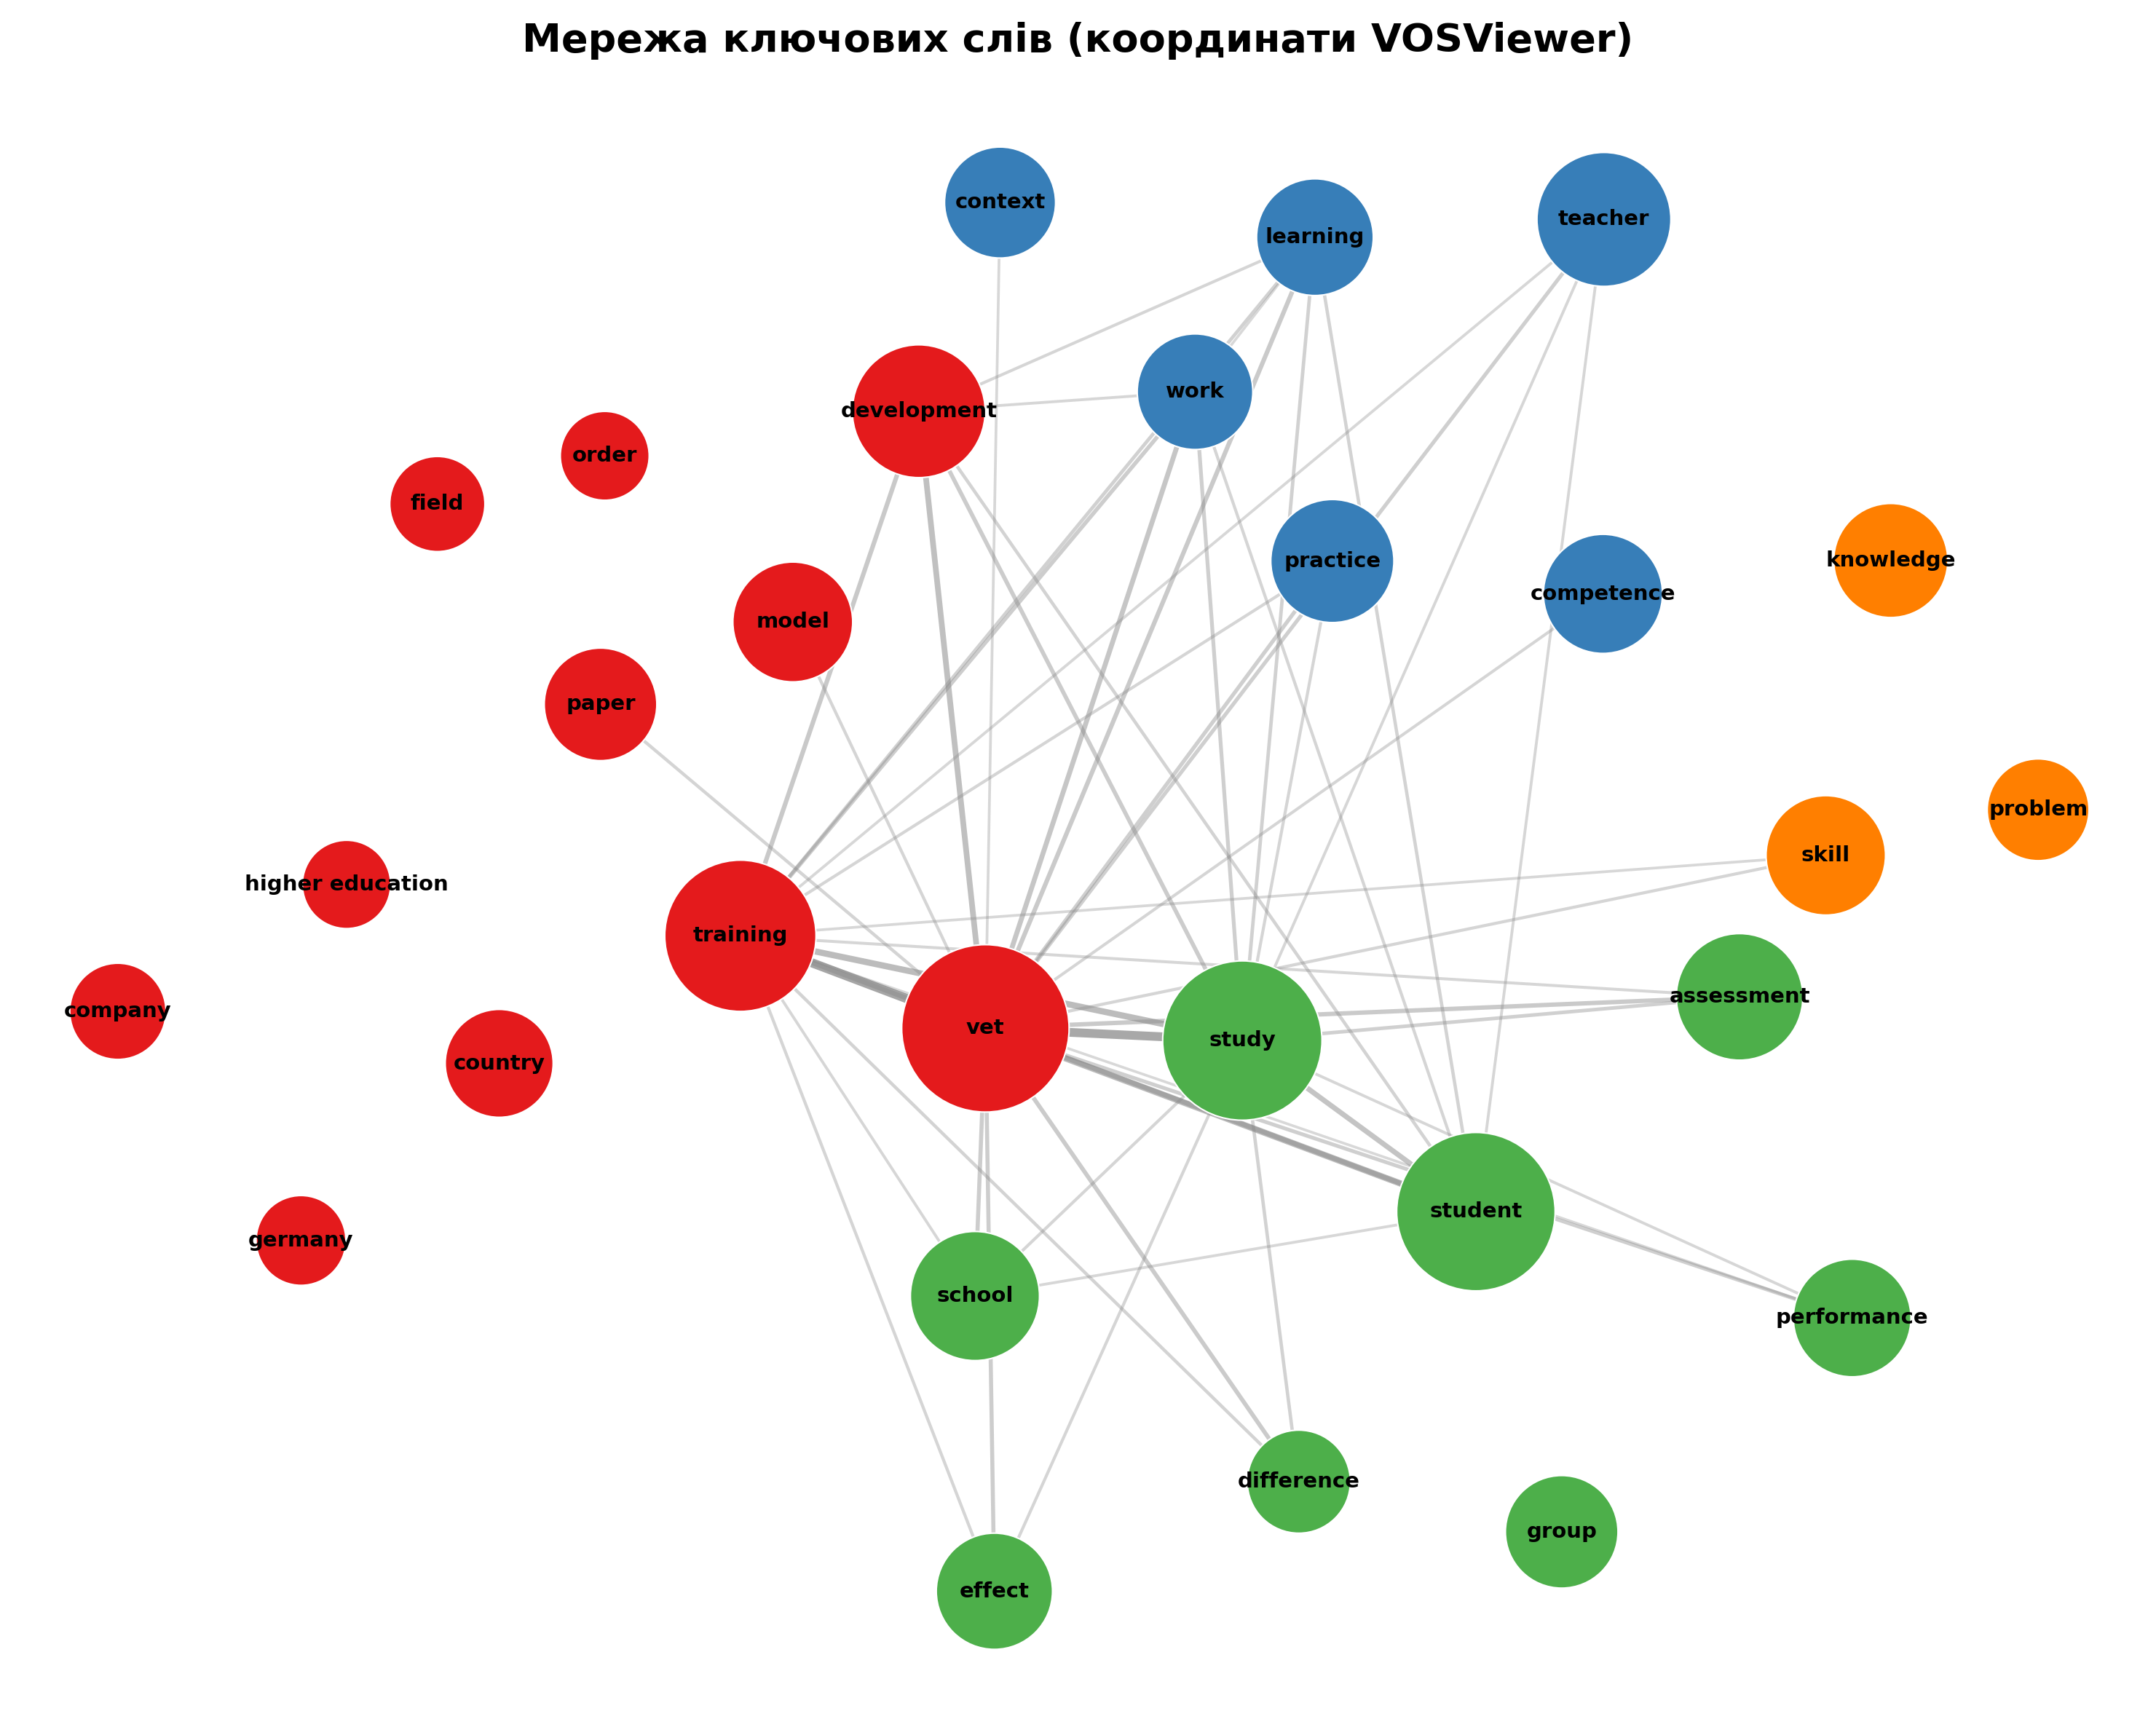
\includegraphics[width=\linewidth]{media/fig_network_vosviewer.png}
    \caption{Мережа ключових слів за координатами VOSViewer.}
    \label{fig:network_vosviewer}
\end{figure}

Накладна карта середнього року публікації (рис.~\ref{fig:overlay_year}) демонструє часову динаміку дослідницького поля. Найновіші теми (жовті відтінки) --- \textit{company} (2019,85), \textit{context} (2019,09), \textit{higher education} (2018,73) --- вказують на зростання уваги до ролі роботодавців, контекстуального навчання та зв'язків ПТО з вищою освітою. Класичні теми (темні відтінки) --- \textit{country} (2016,36), \textit{assessment} (2016,43), \textit{problem} (2016,47) --- відповідають усталеним порівняльним та методологічним підходам.

\begin{figure}[htbp]
    \centering
    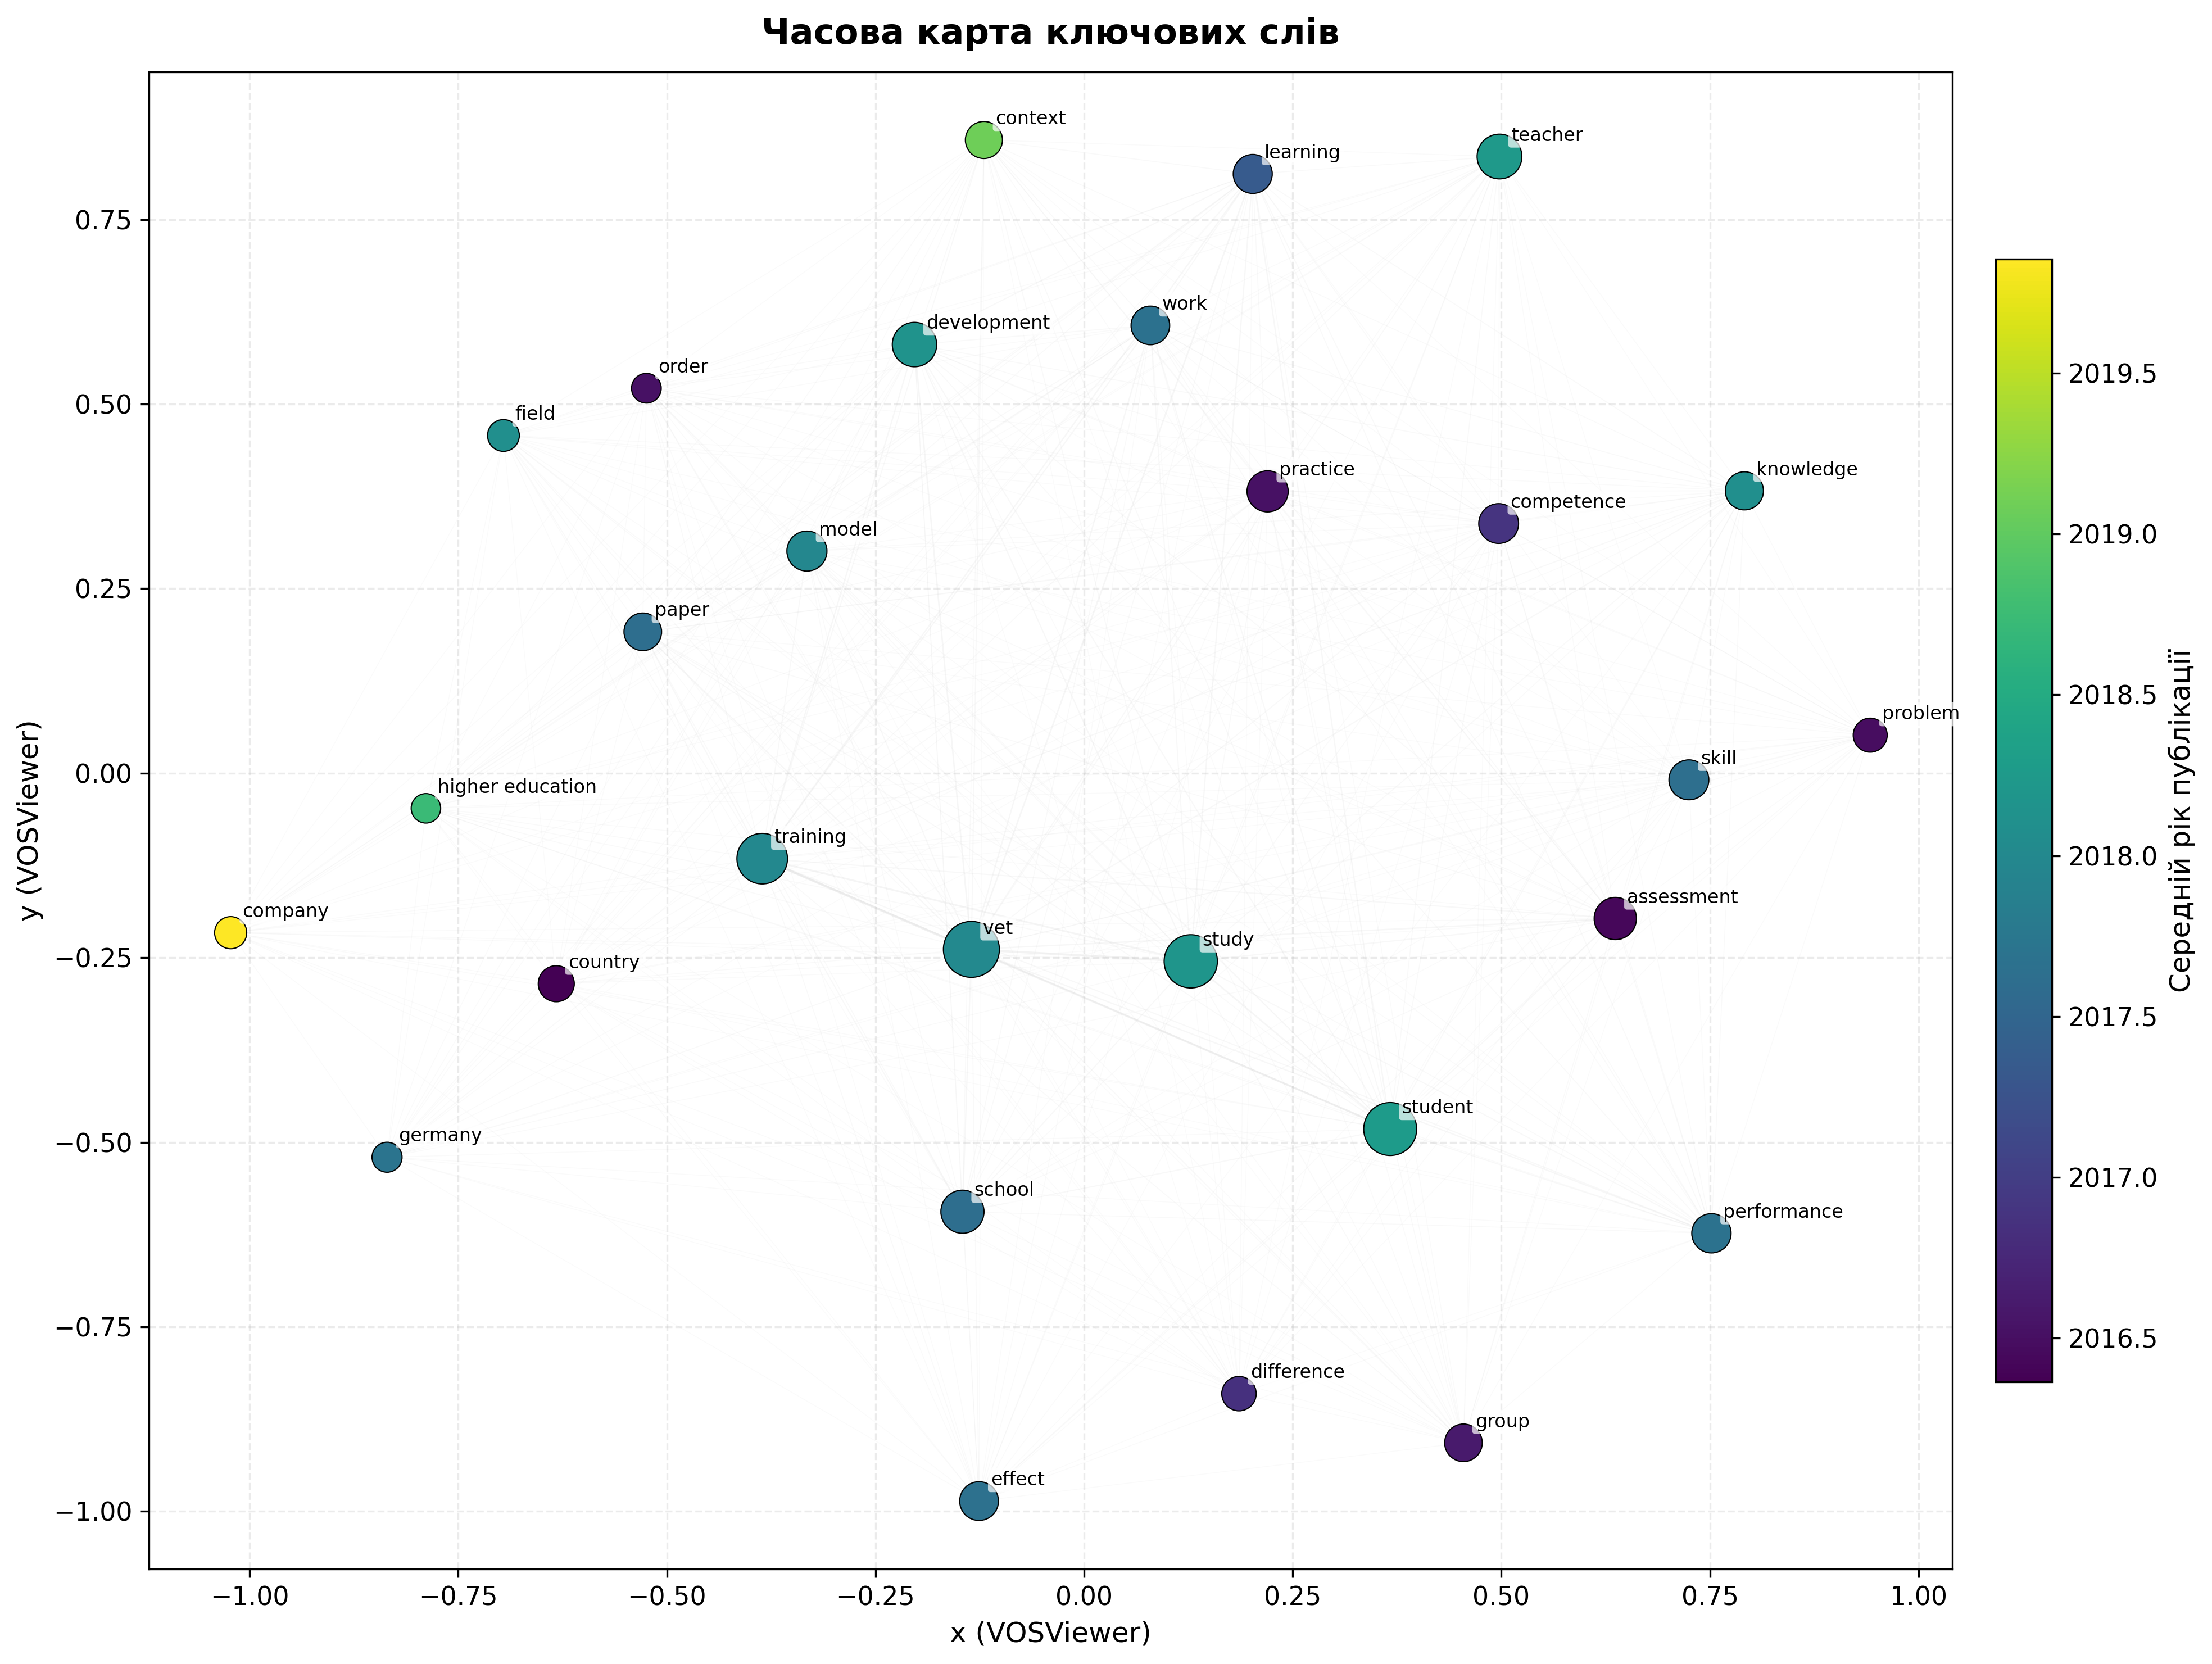
\includegraphics[width=\linewidth]{media/fig_overlay_year.png}
    \caption{Часова карта ключових слів (середній рік публікації).}
    \label{fig:overlay_year}
\end{figure}

Накладна карта середньої цитованості (рис.~\ref{fig:overlay_citations}) показує, що найбільш цитовані терміни --- \textit{competence} (17,04), \textit{germany} (16,31), \textit{effect} (15,88), \textit{difference} (15,79) --- належать до різних кластерів, що свідчить про високий науковий вплив як теоретичних, так і емпіричних досліджень.

\begin{figure}[htbp]
    \centering
    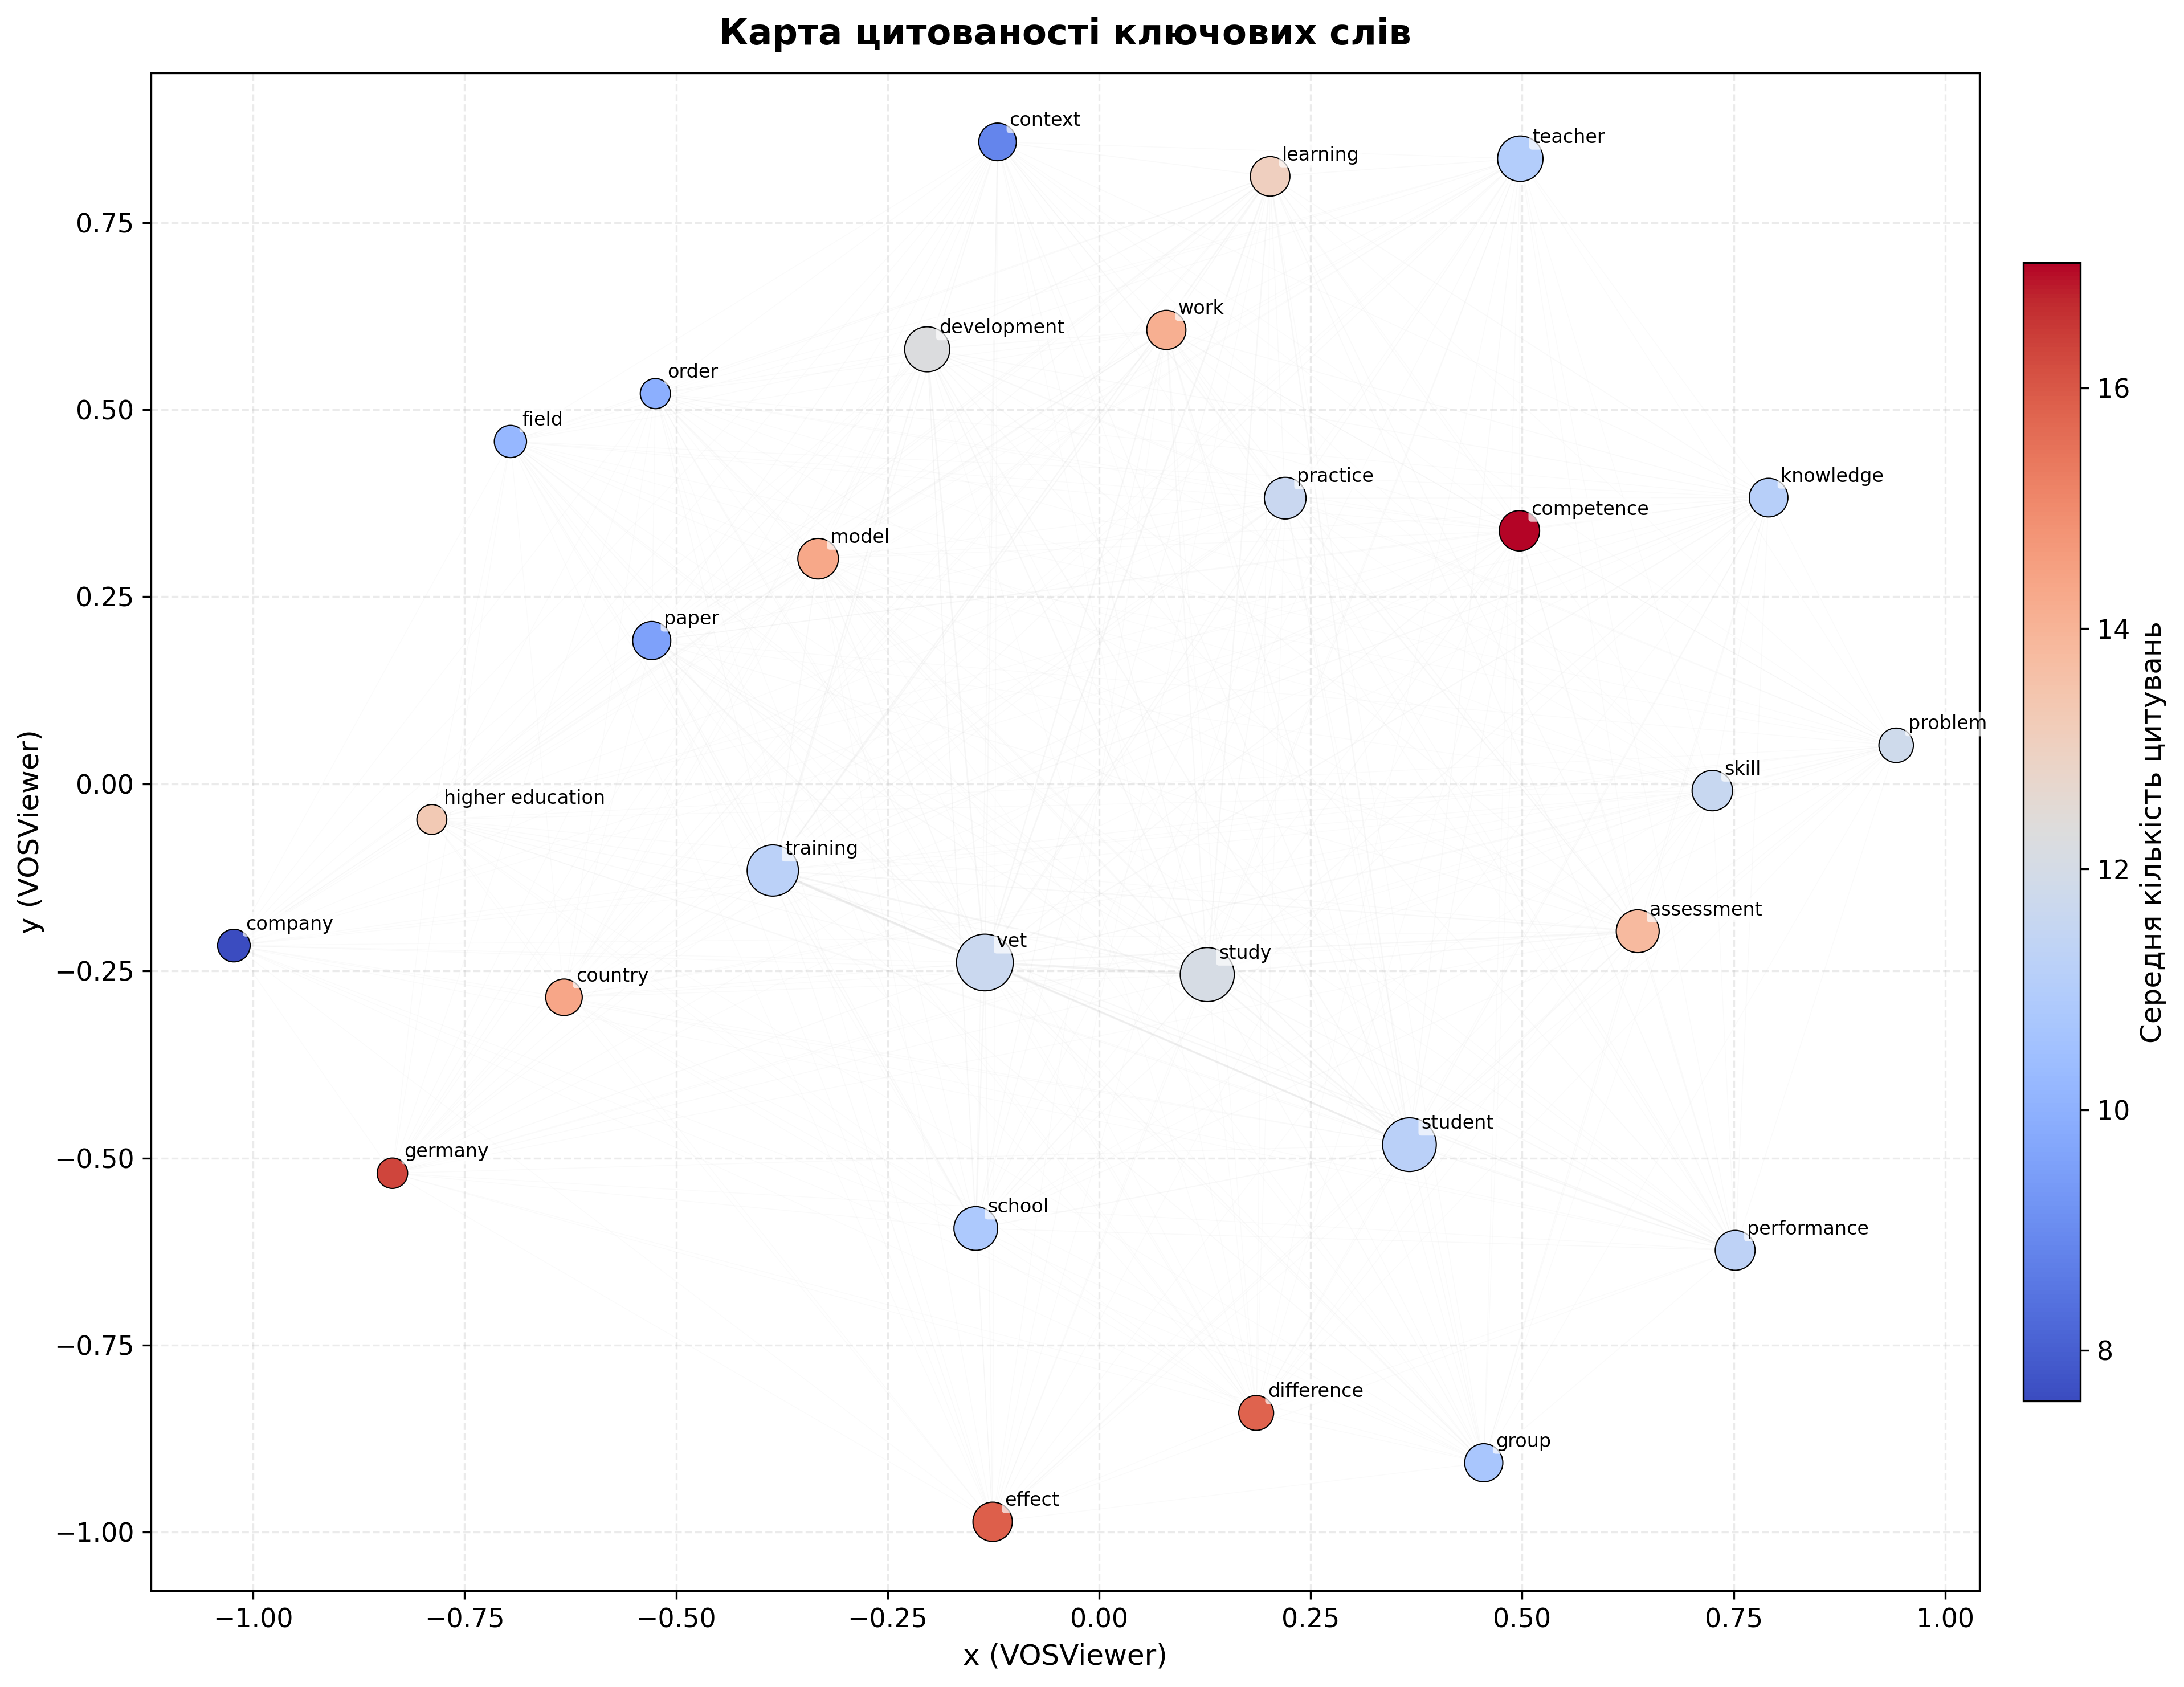
\includegraphics[width=\linewidth]{media/fig_overlay_citations.png}
    \caption{Карта середньої цитованості ключових слів.}
    \label{fig:overlay_citations}
\end{figure}

Карта щільності (рис.~\ref{fig:density}) відображає концентрацію досліджень у семантичному просторі. Найщільніші зони відповідають найбільш активним напрямам досліджень: центральна зона навколо термінів \textit{vet}, \textit{training}, \textit{student}, \textit{study} та зона педагогічної практики навколо \textit{teacher}, \textit{learning}, \textit{competence}.

\begin{figure}[htbp]
    \centering
    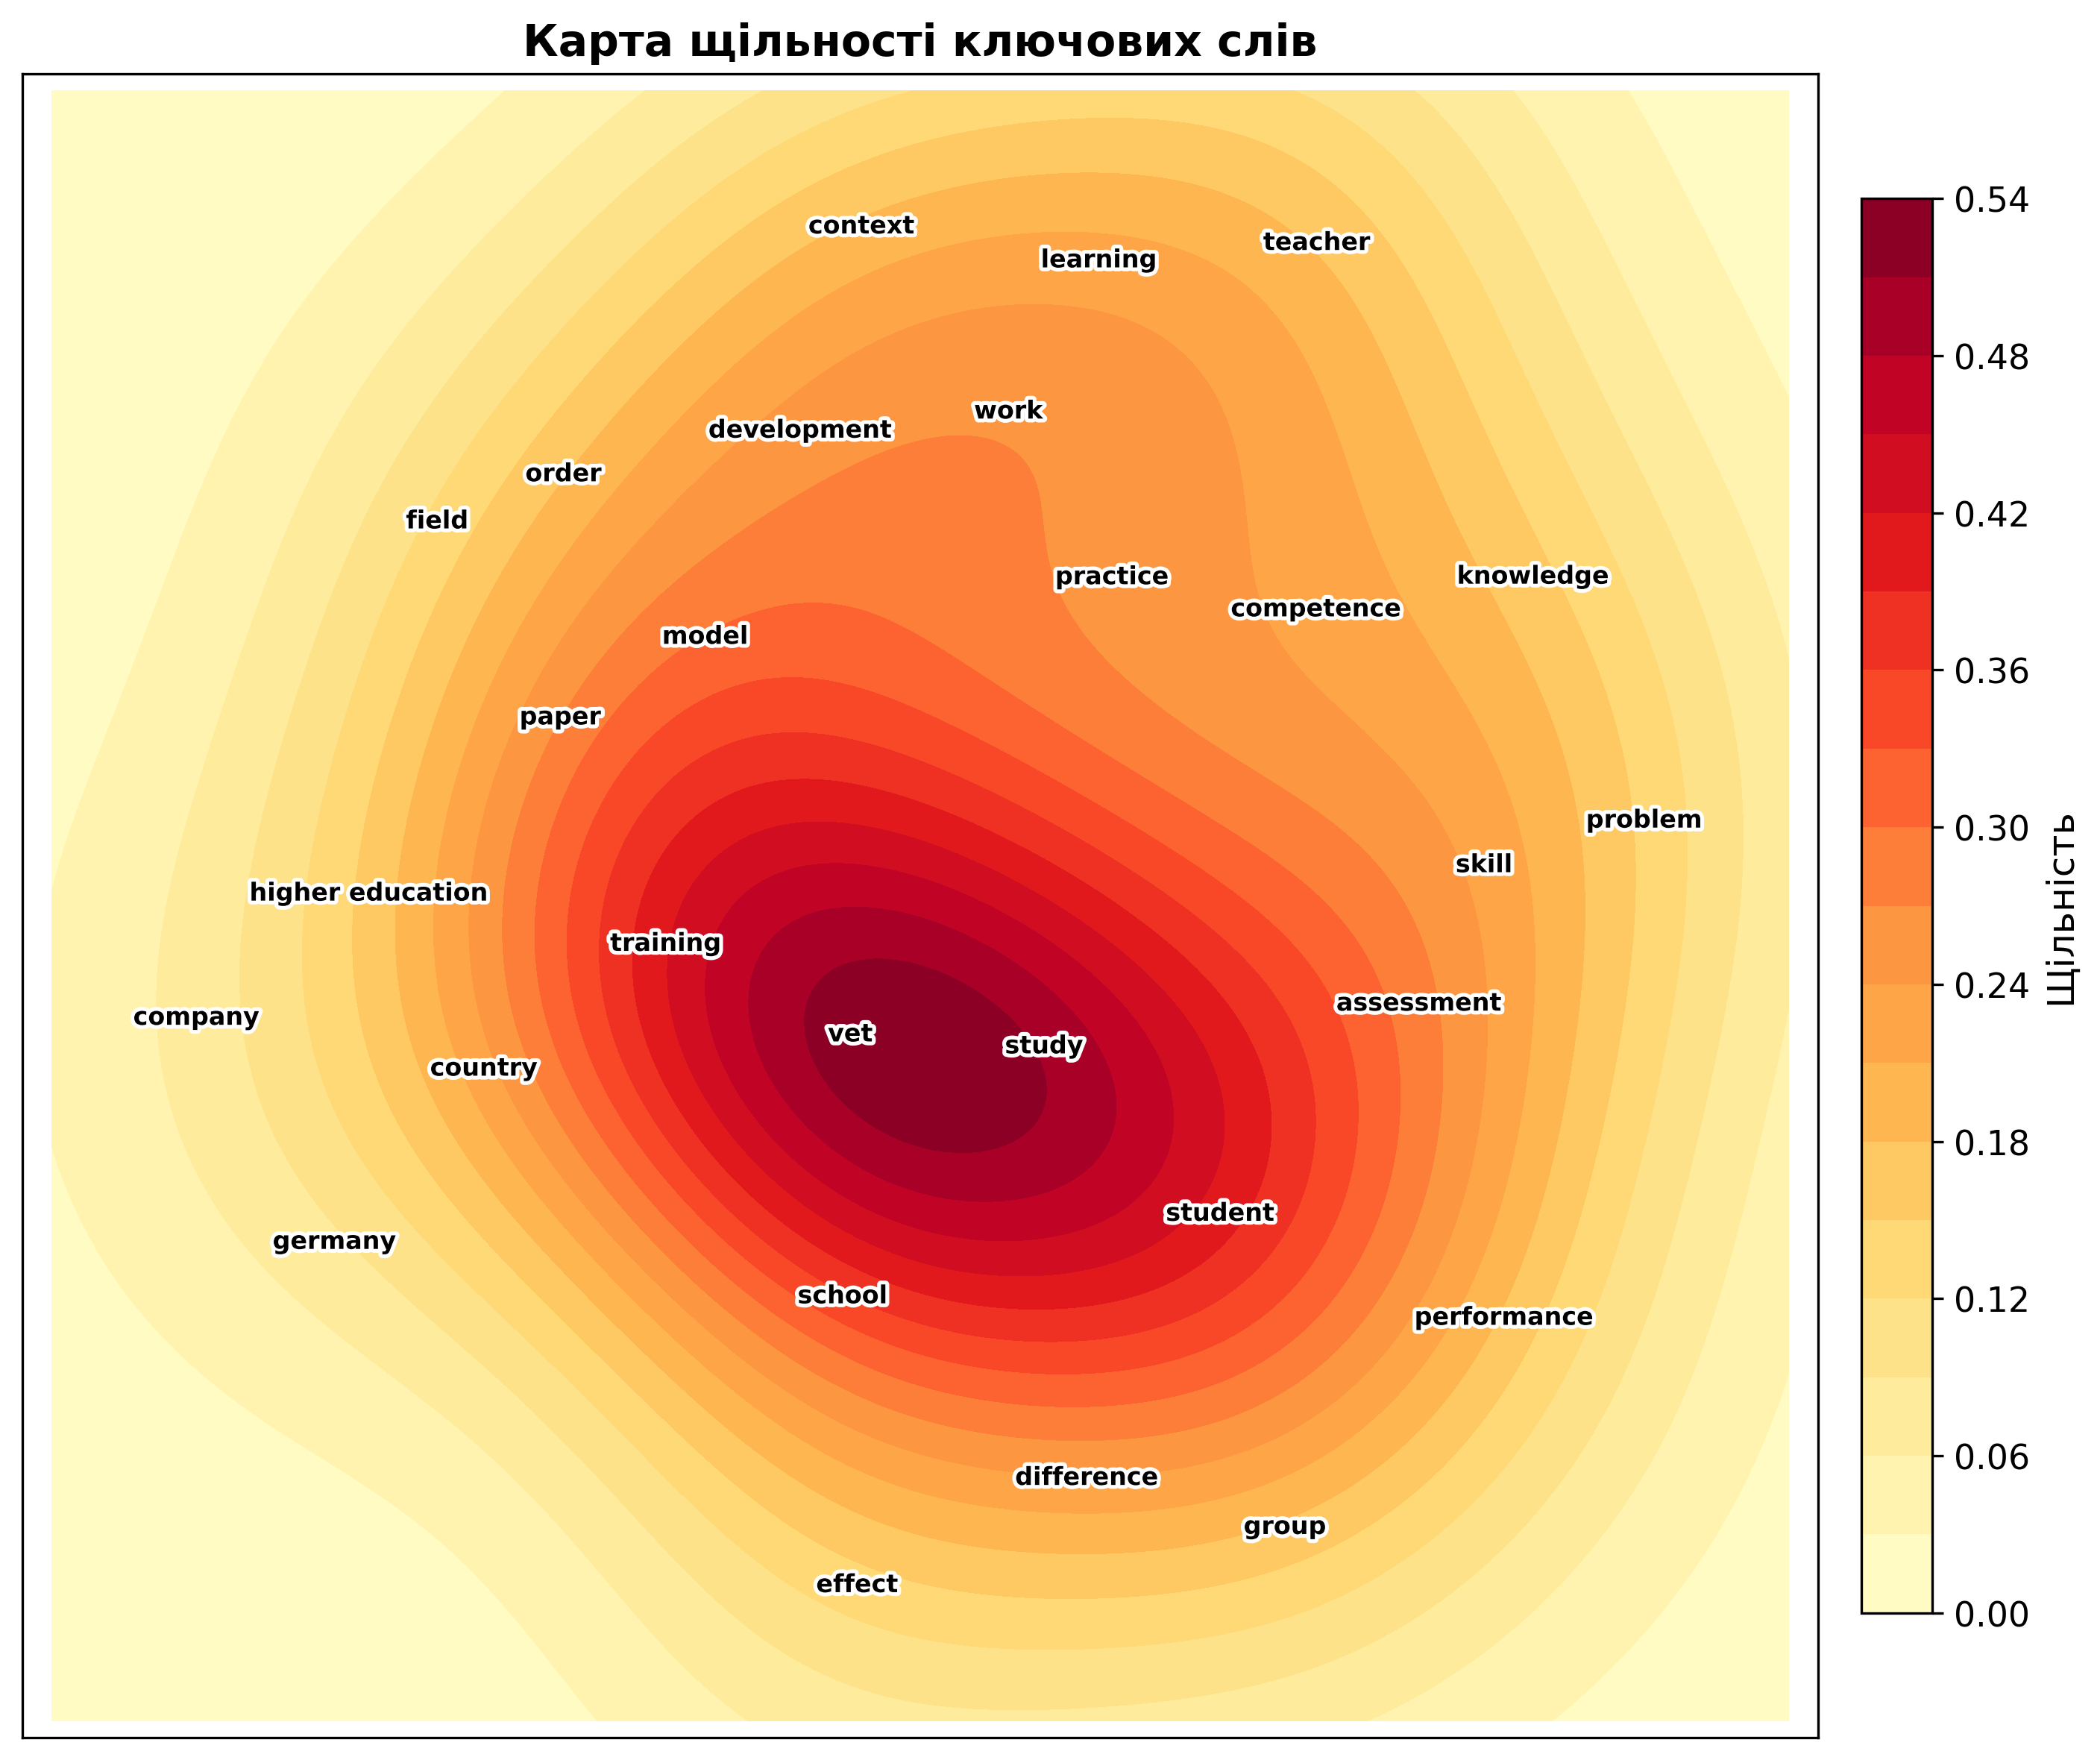
\includegraphics[width=\linewidth]{media/fig_density.png}
    \caption{Карта щільності ключових слів.}
    \label{fig:density}
\end{figure}
